\chapter{Event Related Potential: The P300 Wave}
\label{chapter:six}
\epigraph{Talking off the top of your head....}{Farwell and Donchin}

\section{Introduction}

The P300~\cite{Bashore1991,Farwell1988,Knuth2006} is a positive deflection of the EEG signal which occurs around $300$ ms after the onset of a rare and deviant stimulus that the subject is expected to attend.  It is produced under the oddball paradigm~\cite{WolpawJonathanR2012} and it is consistent across different subjects. It has a lower amplitude  ($\pm 5 \mu V $) compared to basal EEG activity, reaching a Signal to Noise Ratio (SNR) of around $-15$ db estimated based on the amplitude of the P300 response signal divided by the standard deviation of the background EEG activity~\cite{Hu2010}.  

This signal can be cleverly utilized to implement a speller application by means of a Speller Matrix. Farwell and Donchin P300 Speller \cite{Farwell1988} is one the most used BCI paradigms to implement a thought translation device and to send commands to a computer in the form of selected letters, similar to typing on a virtual keyboard.  This procedure exploits this cognitive phenomena by detecting along the EEG trace of a person which is focusing on a sequence of two different visual flashing stimulus, the distinctive P300 transient component each time the expected stimulus flashes.  On the P300 Speller, rows and columns of a 6x6 matrix flash randomly but only the flashing of a column or row where the letter that a user is focusing will trigger concurrently the P300 ERP.

Figure~\ref{fig:p300matrix} shows an example of the Speller Matrix used in the OpenVibe open source software~\cite{Renard2010}, where the flashes of rows and columns provide the deviant stimulus required to elicit this physiological response.   Each time a row or a column that contains the desired letter flashes, the corresponding synchronized EEG signal should also contain the P300 signature and by detecting it, the selected letter can be identified.

\begin{figure}[h!]
\centering
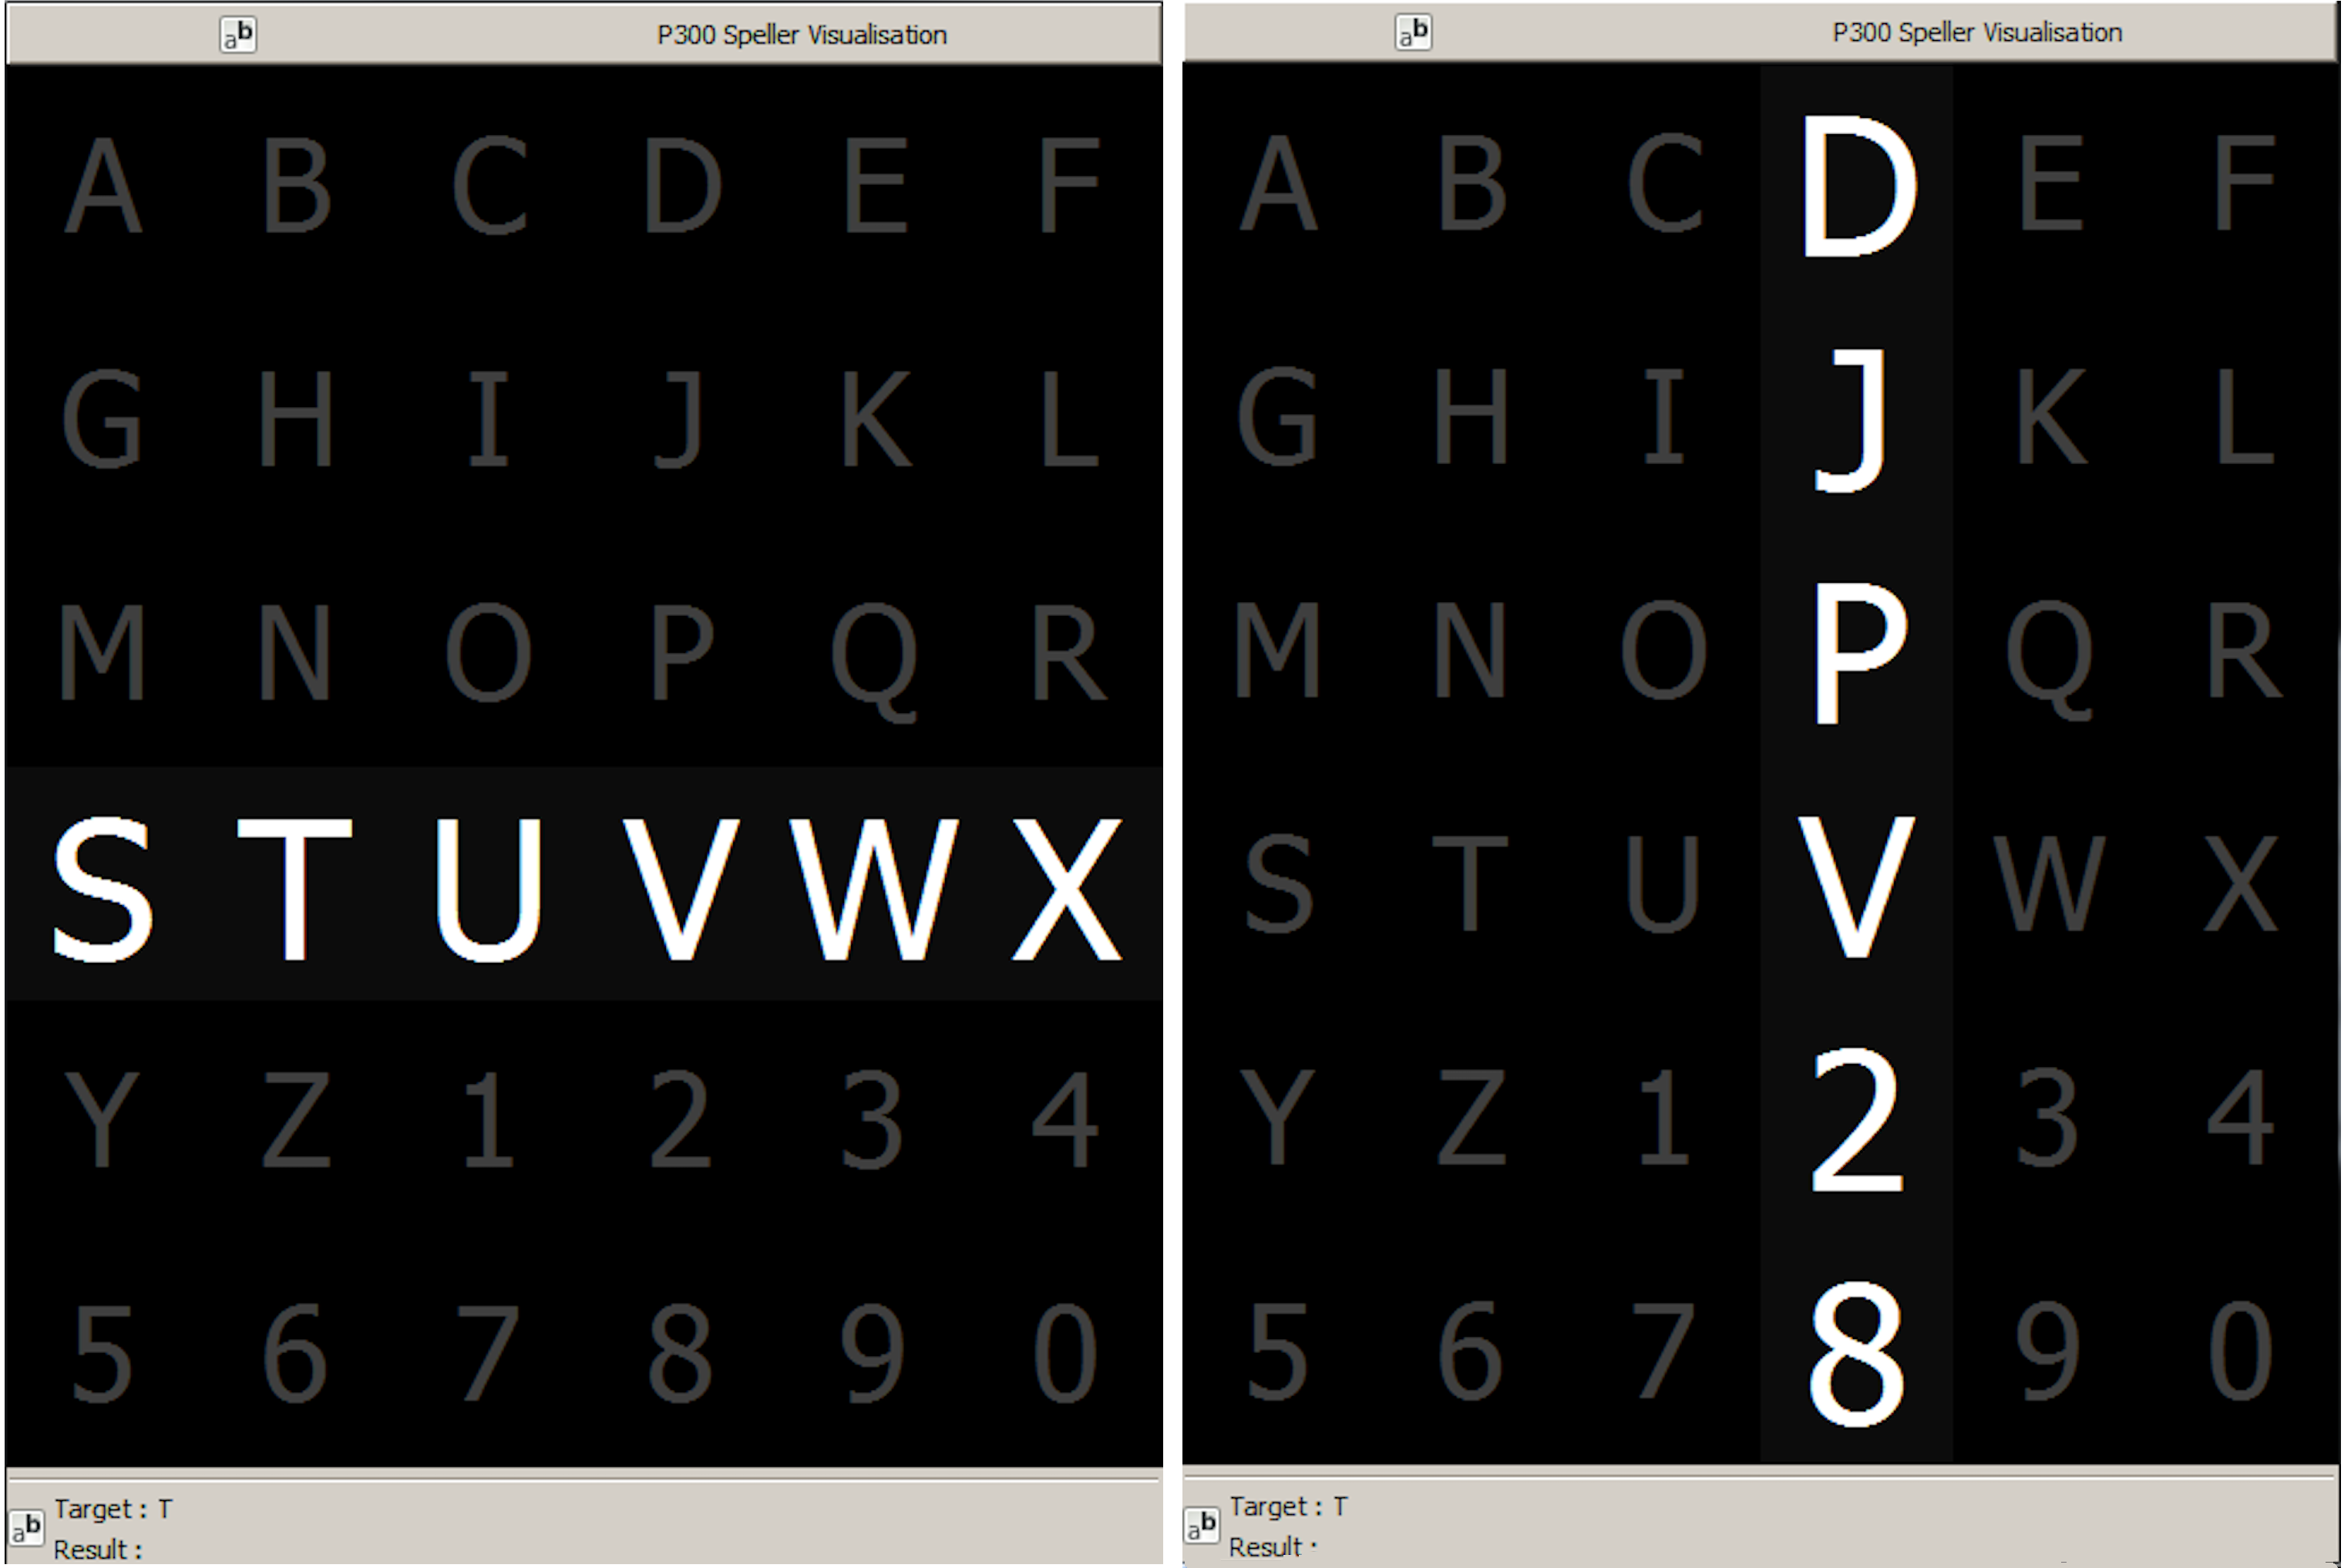
\includegraphics[width=15cm]{images/openvibep300matrix.png}
\caption[P300 Speller Matrix]{Example of the $6 \times 6$ Speller Matrix used in the study obtained from the OpenVibe software.  Rows and columns flash in random permutations.}
\label{fig:p300matrix}
\end{figure}

%In response to this counting, a potential was elicited in the brain.  This response is kown as a P300 wave, as first reported by Sutton.  Detection of the responses an their timing in the measured signal made it possilbe to match rthe responses to one of the rows and one of the columns, and thus, the consen symbol cound be identified.

%TODO bThe flicker Effect (Neuro time series book) and their connection to SSVEP.  Verification of the dataset by means of SSVEP detection.

\section{Materials and Methods}

%TODO Agregar aca que en este caso no queda otra mas que preprocesar la señal debido a que el P300 está muy embebido en la señal.  Ver la figura donde se ve esto bien con el dataset truchado.

In this section, the signal preprocessing, the ERP Extraction, and the Speller Matrix identification are described.  Figure~\ref{fig:classification} outlines a scheme of this process. Additionally, the experiments that were conducted, are also expounded.

\subsection{Preprocessing Pipeline} \label{Pipeline}

Up to this point, EEG signals were treated in \textit{raw} form.  For the signals studied in Chapter~\ref{chapter:four} and \ref{chapter:five} no preprocessing step was necessary. The reason being, the oscillatory processes that are studied contain a waveform that is detected from raw signal plots.  Additionally, for the sake of analyzing waveforms as they are, purposely intensive preprocessing procedure are avoided.  However, this is not the case with the P300 Wave.  The preprocessing step, and more importantly an enhancement of the SNR through signal averaging, is mandatory in order to extract the ERP waveform.

\begin{figure}[htb]
\centering
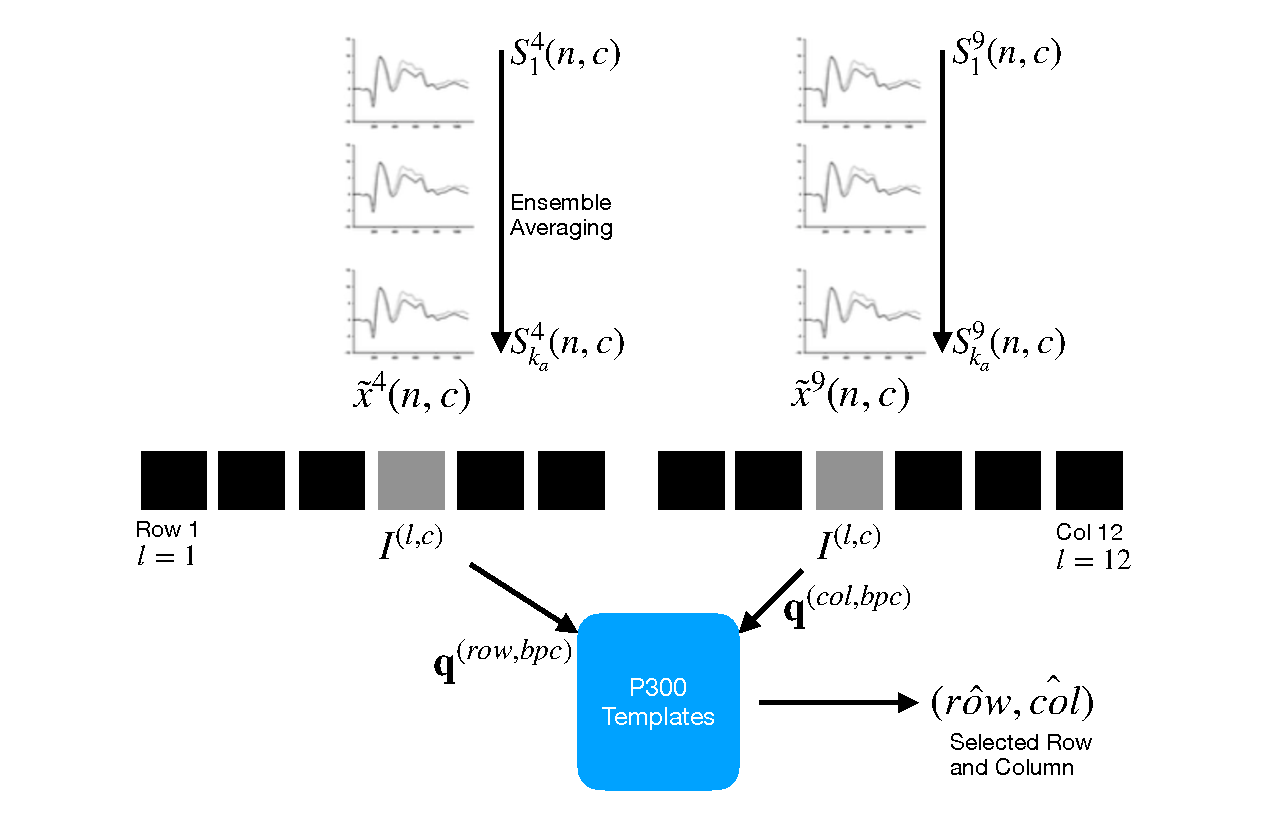
\includegraphics[width=15cm]{images/classificationgraph.pdf}
\caption[P300 Speller Matrix Letter Identification]{For each column and row, an averaged, standardized and scaled signal $\tilde{x}^l(n,c)$ is obtained from the segments $S_i^l$  corresponding to the $\gls{ka}$ intensification sequences with $ 1 \leq i \leq k_a $ and location $l$ varying between $1$ and $12$. From the averaged signal, the image $I^{(l,c)}$ of the signal plot is generated and each descriptor is computed.  By comparing each descriptor $\mathbf{q}$  against the set of templates, the P300 ERP can be detected, and finally the desired letter from the matrix can be inferred.}
\label{fig:classification}
\end{figure}

The data obtained by the capturing device is digitalized and a multichannel EEG signal is constructed. The $6$ rows and $6$ columns of the Speller Matrix are intensified providing the visual stimulus.  The number of a row or column is a location. A sequence of twelve randomly permuted locations $l$ conform an intensification sequence. The whole set of twelve intensifications is repeated $\gls{ka}$ times.

%The multichannel EEG signal is processed on a channel by channel basis.   

\begin{itemize}
\item \textbf{Signal Enhancement}: This stage consists of the enhancement of the SNR of the P300 pattern above the level of basal EEG. The pipeline starts by applying a notch filter to the raw digital signal, a $4$th degree $10$ Hz lowpass Butterworth filter and finally a decimation with a Finite Impulse Response (FIR) filter of order $30$ from the original sampling frequency down to $16$ Hz \cite{Krusienski2006}.  Group delay is accounted for and properly corrected.
\item \textbf{Artifact Removal}: For every complete sequence of $12$ intensifications of $6$ rows and $6$ columns, a basic artifact elimination procedure is implemented by removing the entire sequence when any signal deviates above/bellow $ \pm 70 \mu V $.
\item \textbf{Segmentation}: For each of the $12$ intensifications of one intensification sequence,  a segment $S_{i}^l$  of a window of $\gls{w}$ seconds of the multichannel signal is extracted, starting from the stimulus onset, corresponding to each row/column intensification $l$ and to the intensification sequence $i$. As intensifications are permuted in a random order, the segments are rearranged corresponding to row flickering, labeled 1-6, whereas those corresponding to column flickering are labeled 7-12.  Two of these segments should contain the P300 ERP signature time-locked to the flashing stimulus, one for the row, and one for the column.
\item \textbf{Signal Averaging}: \label{Average}  The P300 ERP is deeply buried under basal EEG so the standard approach to identify it is by point-to-point averaging the time-locked stacked signal segments.  Hence the values which are not related to, and not time-locked to the onset of the stimulus are canceled out~\cite{Liang2008}.  

\begin{story}[Balanced Information Transfer Rate (ITR)]
This signal averaging procedure determines the operation of any P300 Speller.  In order to obtain an improved signal in terms of its SNR,  repetitions of the sequence of row/column intensification are necessary.  And, at the same time, as long as more repetitions are needed, the ability to transfer information faster is diminished, so there is a trade-off that must be acutely determined~\cite{Krusienski2006}.
\end{story}

In brief, the procedure to obtain the point-to-point averaged signal goes as follows:

\begin{enumerate}
\item \label{paso1}Highlight randomly the rows and columns from the matrix.  There is one row and one column that should match the letter selected by the subject.
\item  \label{paso2} Repeat step~\ref{paso1} $\gls{ka}$ times, obtaining the $1 \leq l \leq 12$ segments $S_1^l(n,c),\dots,S_{k_a}^l(n,c)$, of the EEG signal where the variables $1 \leq n \leq N$ and $1 \leq c \leq C$  correspond to sample points and channel, respectively. The parameter $\gls{C}$ is the number of available EEG channels whereas $\gls{N}$ is the segment length and $\gls{Fs}$ is the sampling frequency.  The parameter $\gls{ka}$ is the number of repetitions of intensifications and it is an input parameter of the algorithm.
\item \label{paso3} Compute the Ensemble Average by
\begin{equation}
x^l(n,c)= \frac{1}{k_a}\sum_{i=1}^{k_a}S_i^l(n,c) 
\label{averaging}
\end{equation}  
for $1 \leq n \leq N$ and for the channels $1 \leq c \leq C$. Once this is computed,  the averaged signal $x^l(n,c)$ can be standardized using the procedure from Section~\ref{standardized}, conforming $\tilde{x}^l(n,c)$ for the twelve locations $ 1 \leq l \leq 12$.
\end{enumerate}
\end{itemize}


\subsection{Speller Matrix letter Identification}
\label{Classification}

The speller matrix operation is divided in three parts.  First, the procedure to extract the ERP from EEG signals is detailed.  These ERPs waveforms are represented as descriptors.  Second, these descriptors are used to build the template dictionary $\gls{T}$ during the calibration phase of the speller.  And finally, the spelled letter is identified by extracting descriptors from new signals, and using the classification algorithm to identify them.

\subsubsection{P300 ERP Extraction}
Segments corresponding to row flickering are labeled 1-6, whereas those corresponding to column flickering are labeled 7-12.  The extraction process has the following steps:

\begin{itemize}
%\setcounter{enumi}{3}

\item \textbf{Step A:}\label{pasoa} First highlight rows and columns from the matrix in a random permutation order and obtain the Ensemble Average as detailed in steps~\ref{paso1}, \ref{paso2} and \ref{paso3} in Section \ref{Average}.
\item \textbf{Step B:}\label{paso4} Plot the signals $\tilde{x}^l(n,c)$,  $1 \leq n \leq N$, $1 \leq c \leq C $,  according to Section~\ref{Plot} in order to generate the images $I^{(l,c)}$ for rows and columns $1 \leq l \leq 12$.

\item \textbf{Step C:} Obtain the descriptors $ \mathbf{d}^{(l,c)}$ for rows and columns from $I^{(l,c)}$  in accordance to the method described in Section~\ref{SIFT}. 

\end{itemize}

\subsubsection{Calibration}

A trial, as defined by the BCI2000 platform~\cite{Schalk2004}, is every attempt to select just one letter from the speller.  A set of trials is used for calibration and once the calibration is complete it can be used to identify new letters from new trials.

During the calibration phase, two descriptors $ \mathbf{d}^{(l,c)}$ are extracted for each available channel, corresponding to the locations $l$ of a selection of one previously instructed letter from the set of calibration trials.  These descriptors are the P300 templates, grouped together in the template set $ \gls{T}^c $.   This set is constructed using the steps described in Section \ref{Average} and the steps A, B and C of the P300 ERP extraction process.

Additionally, the best performing channel, $\gls{bpc}$ is identified based on the the channel where the best character recognition rate is obtained.

\subsubsection{Letter identification}

In order to identify the selected letter, the template set $T^{bpc}$ is used as a database.  Thus, new descriptors $\mathbf{q}^{(l,bpc)} $ are computed for each location $l$ and they are compared against the descriptors belonging to the calibration template set $T^{bpc}$.

\begin{itemize}

\item \textbf{Step D:} Match to the calibration template $T^{bpc}$ by computing  

\begin{equation}
\hat{row} = \arg \min_{l \in \{1,\dots,6\}} \sum_{h=1}^{\gls{k}}  {\left\lVert \mathbf{q}^{(l,bpc)} -  \mathbf{d}_{h}^{(bpc)} \right\rVert}  ^{2}
\label{eq:multiclassificationrow}
\end{equation}

\noindent and

\begin{equation}
\hat{col} = \arg \min_{l \in \{7,\dots,12\}} \sum_{h=1}^{\gls{k}}  {\left\lVert \mathbf{q}^{(l,bpc)} -  \mathbf{d}_{h}^{(bpc)} \right\rVert}  ^{2}
\label{eq:multiclassificationcol}
\end{equation}

\noindent with $\mathbf{d}_{h}^{(bpc)}$ belonging to the set $N_T( \mathbf{q}^{(l,bpc)}  )$, which is defined as $N_T(\mathbf{q}^{(l,bpc)} ) = \{ \mathbf{d}_{h}^{(bpc)} \in T^{bpc} /  \mathbf{d}^{(bpc)} $  is the $\gls{k}$-nearest neighbor of $ \mathbf{q}^{(l,bpc)} \}$ for the best performing channel.  This procedure is a unary classification scheme, an adapted version of the algorithm described in Section~\ref{nbnn} to the letter identification required in the BCI-Based P300 Speller implementation.

\end{itemize}
By computing the aforementioned equations, the letter of the matrix can be determined from the intersection of the row $ \hat{row} $ and column $ \hat{col} $. 
Figure~\ref{fig:classification} shows a scheme of this process. 


\subsection{Experimental Protocol} \label{Protocol}

%In the following sections the characteristics of the datasets and parameters of the identification algorithm are described. 

To verify the validity of the proposed framework and method over transients events, experiments over four different datasets are performed.  The first three datasets use a similar experimentation protocol, whereas the last one is from a BCI Competition.

First, the public dataset 008-2014~\cite{Riccio2013} published on the BNCI-Horizon website~\cite{Brunner2014} by  IRCCS Fondazione Santa Lucia, is used. A BCI Simulation is performed to decode the spelled words from the provided signals.

Additionally, an own dataset with the same experimental conditions is generated.  A different BCI Simulation is implemented and the decoding of letters is performed. 

In order to verify how this method performs against other similar methods that also use the structure of the waveform, a pseudo-real dataset is constructed where the characteristics of the ERP are carefully adjusted simulating different cognitive mechanisms that can alter their shape.

Finally, the performance of the method presented in this Thesis is tested against one of the dataset published by the BCI Competitions. 

\subsubsection{Dataset I - P300 ALS Public Dataset} \label{ALSDataset}

The experimental protocol used to generate this dataset is explained in~\cite{Riccio2013} but can be summarized as follows:  8 subjects with confirmed diagnoses but on different stages of ALS disease, were recruited and accepted to perform the experiments. The Visual P300 detection task designed for this experiment consisted of spelling 7 words of 5 letters each, using the traditional P300 Speller Matrix~\cite{Farwell1988}. The flashing of rows and columns provide the deviant stimulus required to elicit this physiological response.  The first 3 words are used for calibration and the remaining 4 words, for testing with visual feedback.  A trial is every attempt to select a letter from the speller. It is composed of signal segments corresponding to $k_a =10$ repetitions of flashes of 6 rows and $k_a =10$ repetitions of flashes of 6 columns of the matrix, yielding 120 repetitions.  Flashing of a row or a column is performed for 0.125 s, following by a resting period (i.e. inter-stimulus interval) of the same length.  After 120 repetitions an inter-trial pause is included before resuming with the following letter.

The recorded dataset was sampled at 256 Hz and it consisted of a scalp multichannel EEG signal for electrode channels Fz, Cz, Pz, Oz, P3, P4, PO7 and PO8, identified according to the 10-20 International System,  for each one of the 8 subjects.   The recording device was a research-oriented digital EEG device (g.Mobilab, g.Tec, Austria) and the data acquisition and stimuli delivery were handled by the BCI2000 open source software~\cite{Schalk2004}.

In order to assess and verify the identification of the P300 response, subjects are instructed to perform a copy-spelling task. They have to fix their attention to successive letters for copying a previously determined set of words, in contrast to a free-running operation of the speller where each user decides on its own what letter to choose.

\subsubsection{Dataset II - P300 for healthy subjects}
\label{P300healthysubject}

We replicate the same experiment on healthy subjects using a wireless digital EEG device (g.Nautilus, g.Tec, Austria).  Figure~\ref{fig:gtecdevice} shows the front and back of the g.Tec head cap and two subjects performing this experiment.   The experimental conditions are the same as those used for the previous dataset, as detailed in section~\ref{ALSDataset}.  The produced dataset is available in a public online repository~\cite{owndataset}.

Participants are recruited voluntarily and the experiment is conducted anonymously in accordance with the Declaration of Helsinki published by the World Health Organization.  No monetary compensation is handed out and all participants agree and sign a written informed consent.  This study is approved by the \textit{Departamento de Investigación y Doctorado, Instituto Tecnológico de Buenos Aires (ITBA)}.  All healthy subjects have normal or corrected-to-normal vision and no history of neurological disorders. The experiment is performed with 8 subjects, 6 males, 2 females, 6 right-handed, 2 left-handed, average age 29.00 years, standard deviation  11.56 years, range 20-56 years.

EEG data is collected in a single recording session. Participants are seated in a comfortable chair, with their vision aligned to a computer screen located one meter in front of them.  The handling and processing of the data and stimuli is conducted by the OpenVibe platform~\cite{Renard2010}. 

Gel-based active electrodes (g.LADYbird, g.Tec, Austria) are used on the same positions Fz, Cz, Pz, Oz, P3,P4, PO7 and PO8.  Reference is set to the right ear lobe and ground is preset as the AFz position.   Sampling frequency is slightly different, and is set to 250 Hz, which is the closest possible to the one used with the other dataset.

%Fz, Cz, P3, Pz, P4, PO7, PO8 and Oz. 

%8 gel-based active electrodes (g.LADYbird) + g.LADYbird (GND) + g.GAMMAearclip (REF) C3, Cz, C4, CPz, P3, Pz, P4, POz, GND: AFz, REF: right ear

\begin{figure}[H]
\centering
\subfigure[Front view of g.LADYbird cap showing three frontal electrodes AFz, Fz and Cz.]
{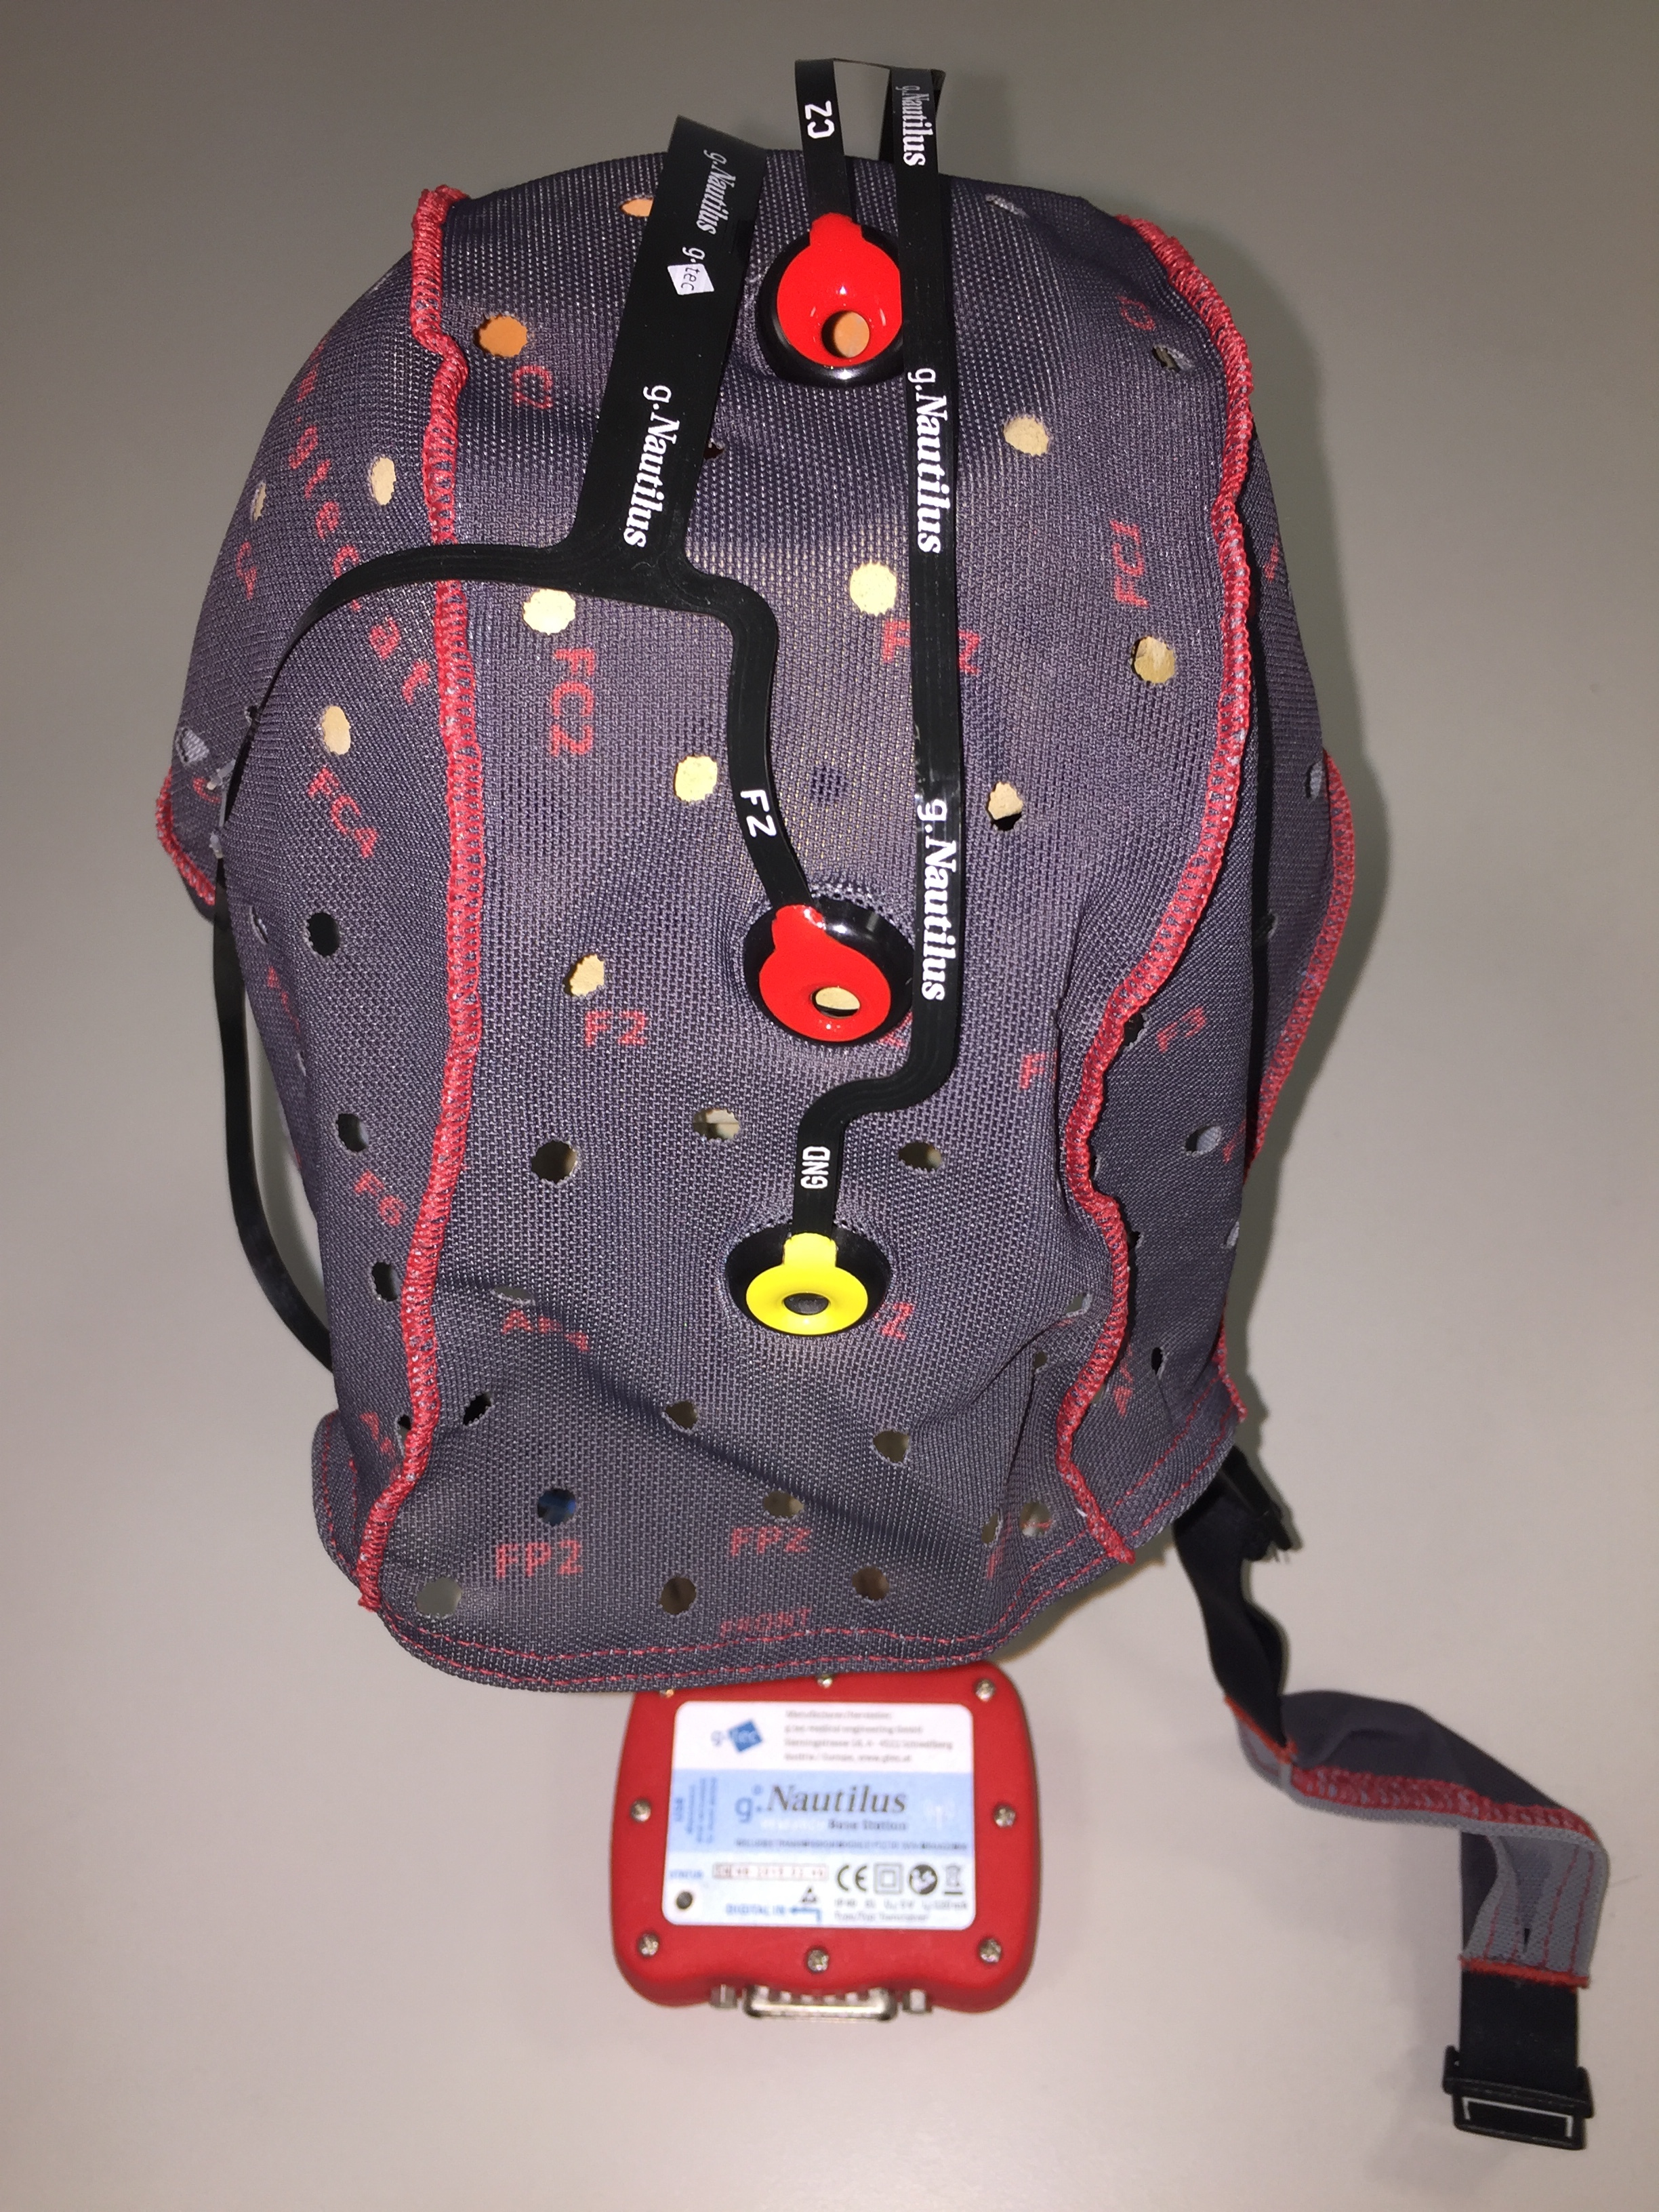
\includegraphics[width=.45\linewidth]{images/gTecfront.jpg}}
\subfigure[Rear view of g.LADYbird cap showing Cz and Pz electrodes.]
{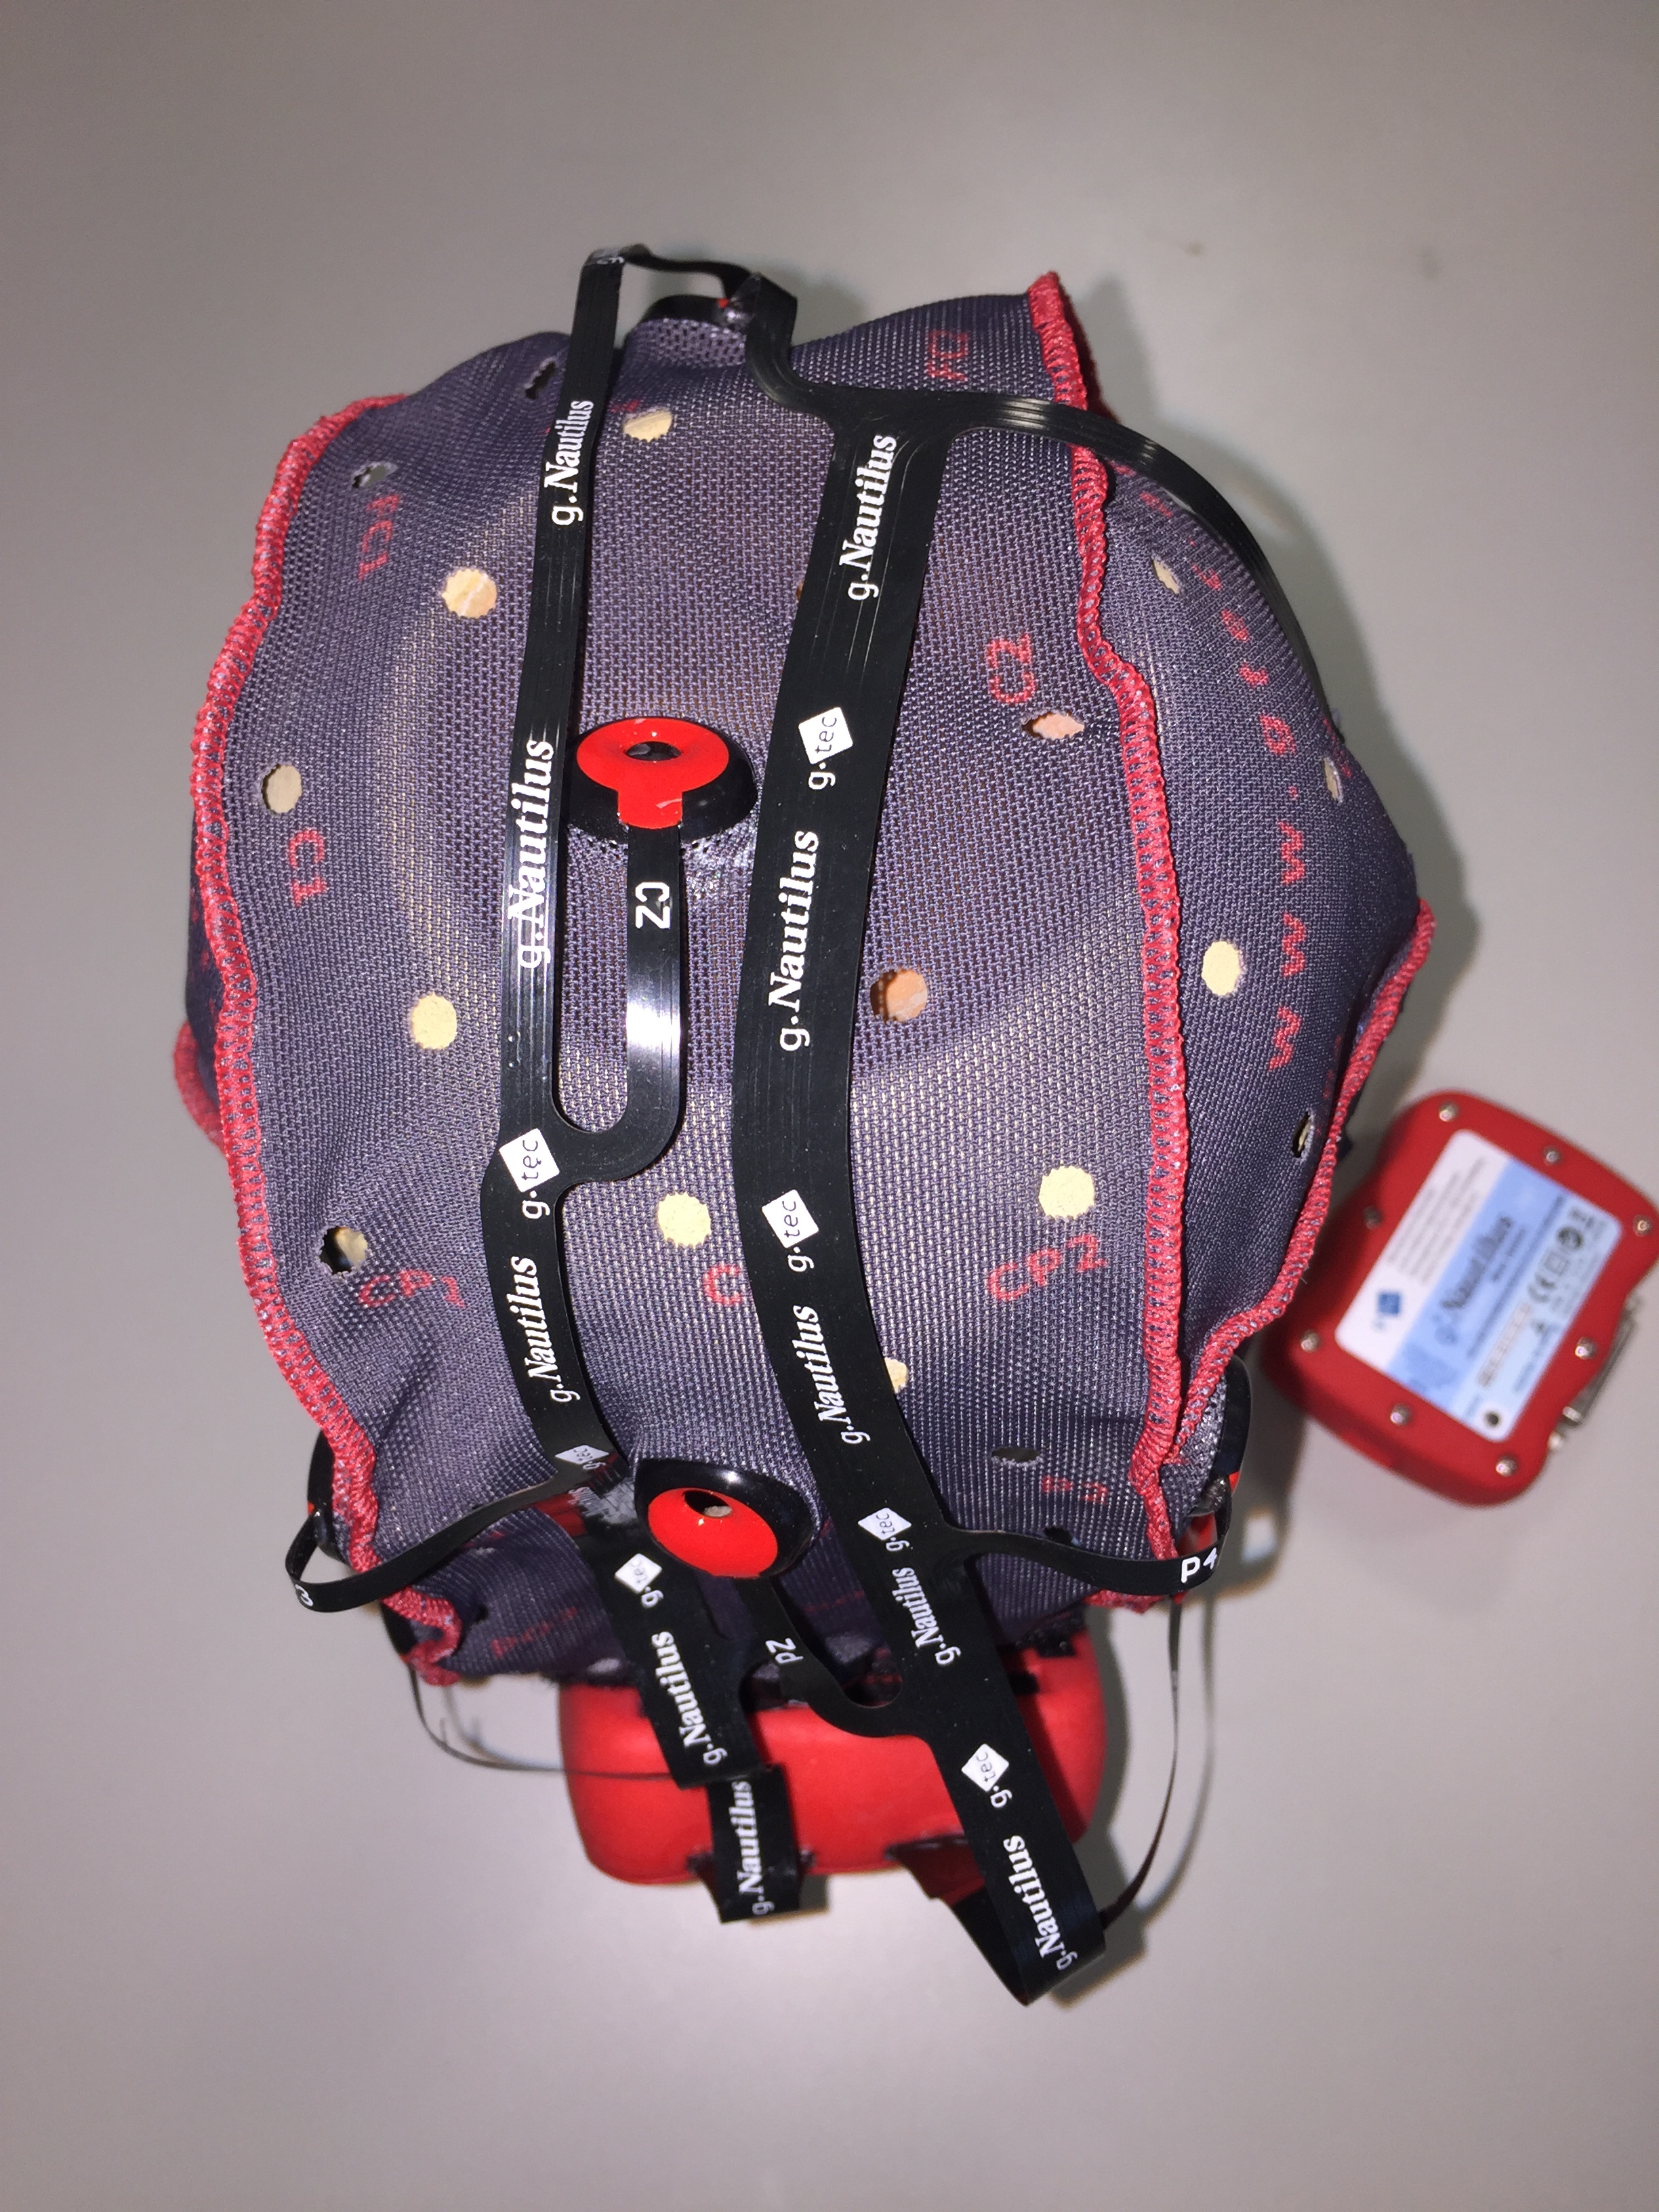
\includegraphics[width=.45\linewidth]{images/gTecback.jpg}}
\subfigure[Subject performing the experiment described in section \ref{P300healthysubject}.]
{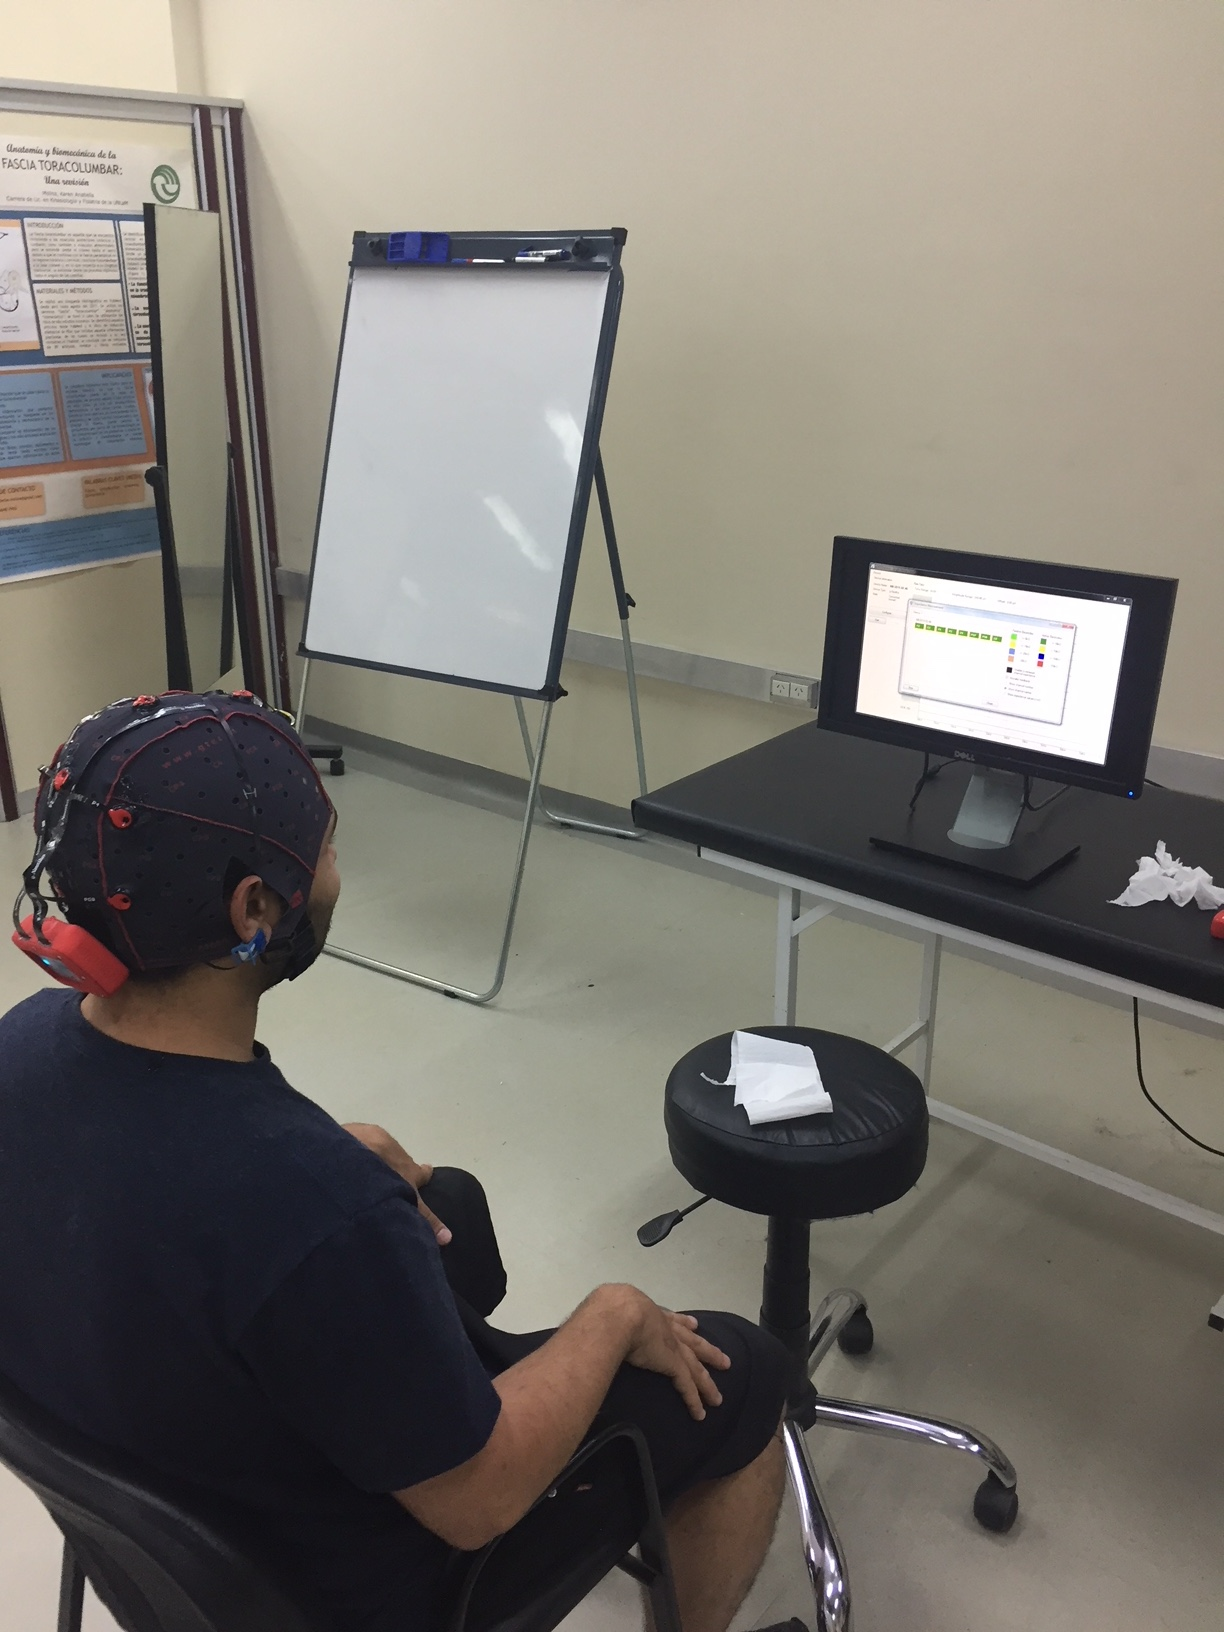
\includegraphics[width=.45\linewidth]{images/gTecsubject2.jpg}}
\subfigure[A different subject performing the P300 Speller experiment.]
{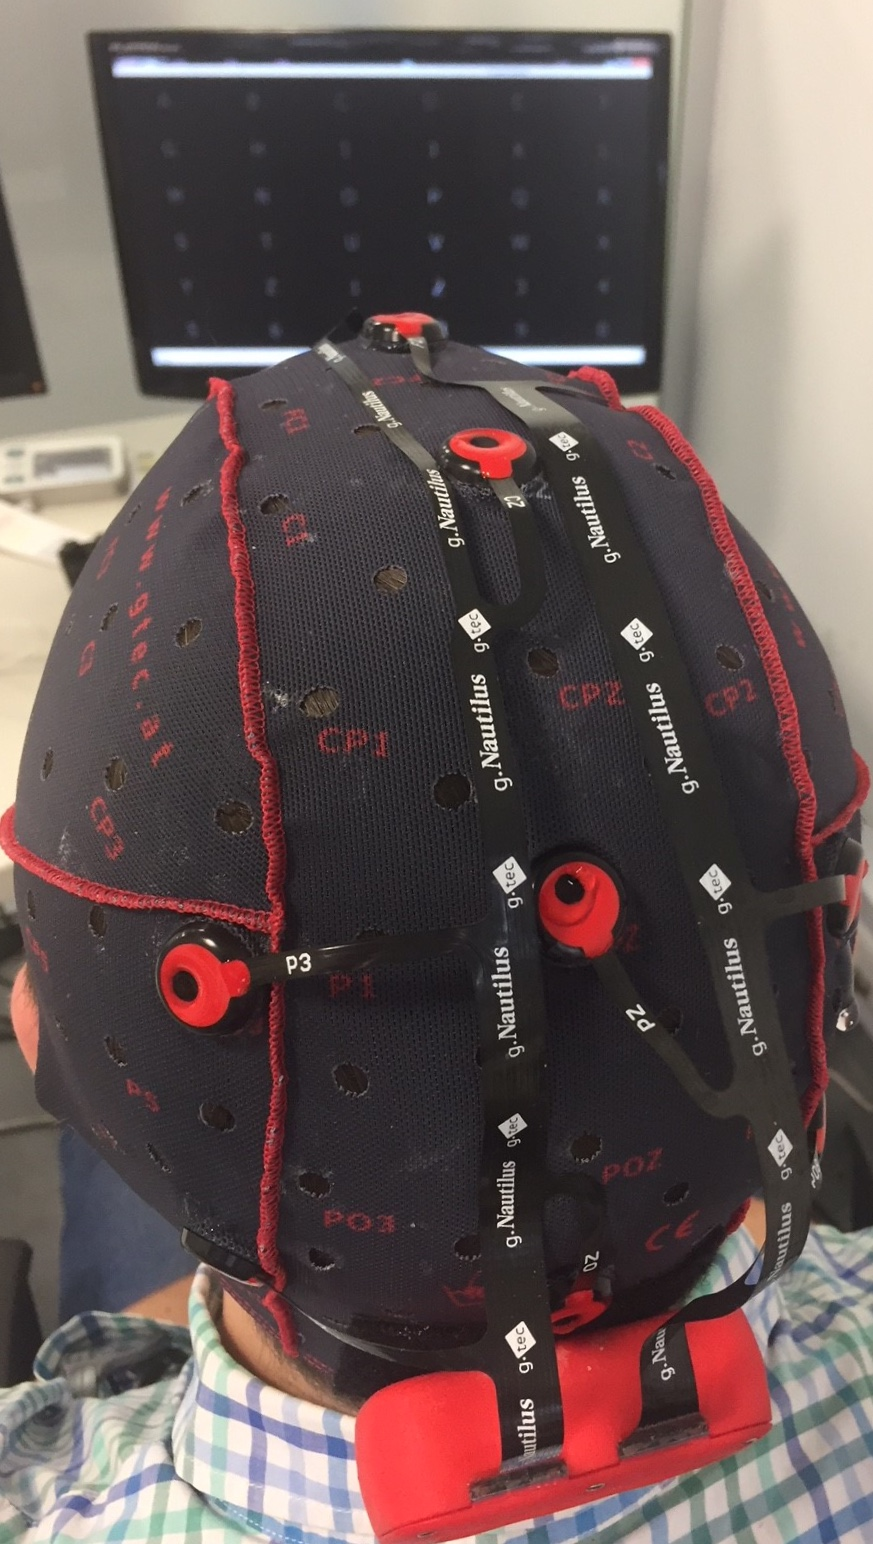
\includegraphics[height=260pt,width=.45\linewidth]{images/gTecsubject3.jpg}}
\caption[g.Tec Device]{The g.Tec device, wearable and wireless g.Nautilus headset. Subjects wearing the g.LADYbird cap. }
\label{fig:gtecdevice}
\end{figure}

\subsubsection{Dataset III - P300 Pseudo-Real Dataset Generation}

To construct this artificial dataset, a P300 ERP template, obtained from the ALS patients dataset, is superimposed into a distinct EEG stream with null-signals.  This EEG trace was experimentally obtained by a subject which was observing the flashing of the stimulus matrix during a P300 Speller procedure but did not engage in focusing on any letter in particular. Everything is there, except the P300 ERP component. Along the EEG stream, the markers information was used to localize the \textit{True} segments where the P300 should have been found, and those timing locations are used to superimpose the extracted ERP waveform.  By implementing this pseudo-real approach, it is possible to effectively control null-signals and to adjust the shape of this evoked potential in accordance to similar procedures used in other works \cite{Ouyang2017,Jaskowski2000,QuianQuiroga2003}.

The template ERP is acquired from the Subject Number $8$ of the public dataset 008-2014 of ALS patients.  Segments from the EEG signal containing the ERP are extracted for the trial number $2$, and they are point-to-point coherently averaged.  This P300 ERP can be seen in Figure~\ref{fig:erptemplate1}. 

\begin{figure}[h!]
\centering
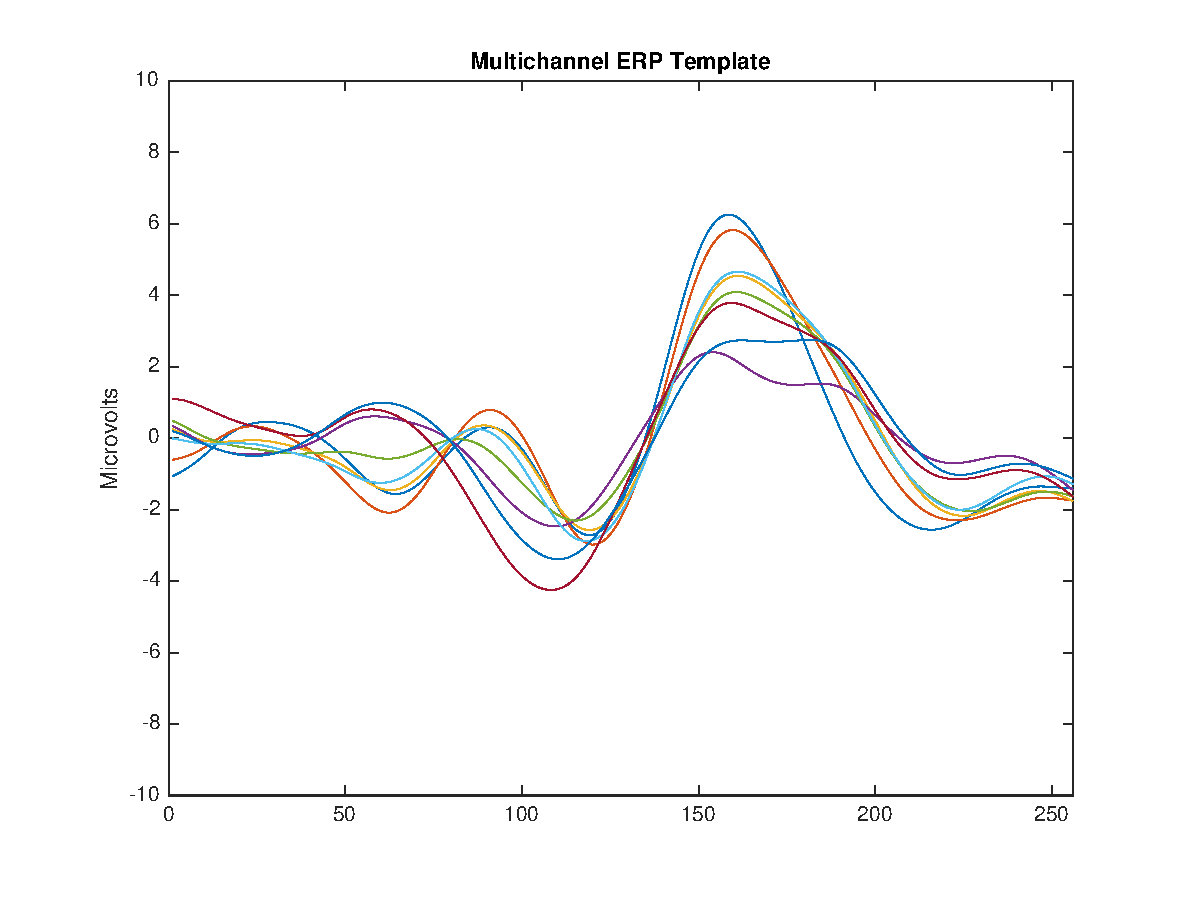
\includegraphics[width=12cm]{images/erptemplate1.eps}
\caption[P300 ERP Template]{ERP Template obtained from the coherent point-to-point ensemble average from the signals of Subject Eight of the BNCI Horizon public dataset 008-2014. The template is $1$-second long which is 256 sample points, and the eight channels are superimposed with different colors.  Vertical axis represents amplitude in $\mu V$ while horizontal axis reflects discrete sample points. The P3b component can be seen around the sample index $150$ and $200$.}
\label{fig:erptemplate1}
\end{figure}

The EEG stream with null-P300 signal is obtained by the following procedure: 
A subject participant is recruited voluntarily and the experiment is conducted anonymously in accordance with the Declaration of Helsinki published by the World Health Organization.  No monetary compensation is handed out and she/he agrees and signs a written informed consent.  This study is approved by the \textit{Departamento de Investigación y Doctorado, Instituto Tecnológico de Buenos Aires (ITBA)}.  The participant is healthy and have normal or corrected-to-normal vision and no history of neurological disorders. This voluntary subject is aged between 20-30 years old.  EEG data is collected in a single recording session. She/He is seated in a comfortable chair, with her/his vision aligned to a computer screen located one meter in front of her/him.  The handling and processing of the data and stimuli is conducted by the OpenVibe platform~\cite{Renard2010}.  Gel-based active electrodes (g.LADYbird, g.Tec, Austria) are used on locations Fz, Cz, Pz, Oz, P3,P4, PO7 and PO8 according to the 10-20 international system.  Reference is set to the right ear lobe and ground is preset as the AFz position.   Sampling frequency is set to 250 Hz.

The participant is instructed to passively watch the flashing screen while not focusing on any particular letter.  The experimental conditions are the same as those described for previous datasets.  A questionnaire is handed out at the end of the experiment with questions about how the participant felt during it, without giving more details.  

%This P300 Speller protocol consist in the flashing of 35 trails of 35 letters (7 words of 5 letter) where the intensification sequence of 6 rows and 6 columns is repeated 10 times for each letter.  More details can be found on the published work of \cite{Riccio2013}.

Figure~\ref{fig:gains} shows a $5s$ sample of the EEG trace obtained with the MNE library~\cite{Gramfort2013}.  Channel $S$ represents the twelve different stimulus markers (columns or rows) while channel $L$ represent the label (\textit{True} vs \textit{False}).  Labels are represented by square signals.  \textit{False} segments are marked with single amplitude square signals while \textit{True} segments are identified by double-amplitude square signals.  Subfigure (a) shows the signals before the ERP template is superimposed while subfigure (b) shows the same signals with the superimposed ERP template.  At first-sight, differences are really hard to spot visually.  Subfigures (c) and (d) show only one second of channels Cz and L from the same segment.  The superimposed ERP can be devised enclosed by the vertical bars, around $31.5$s, where in (d) the peak is slightly bigger.  Figure~\ref{fig:gaincheck} shows the obtained ensemble average ERPs as result of superimposing the template signal into the EEG stream, time-locked to the stimulus onset.   These 12 point-to-point averaged segments correspond to the first trial of the EEG stream.

%The original signal-to-noise ratio was calculated as Hue 2010.

\begin{figure}[h!]
\centering
\subfigure[EEG trace of the original signal.]{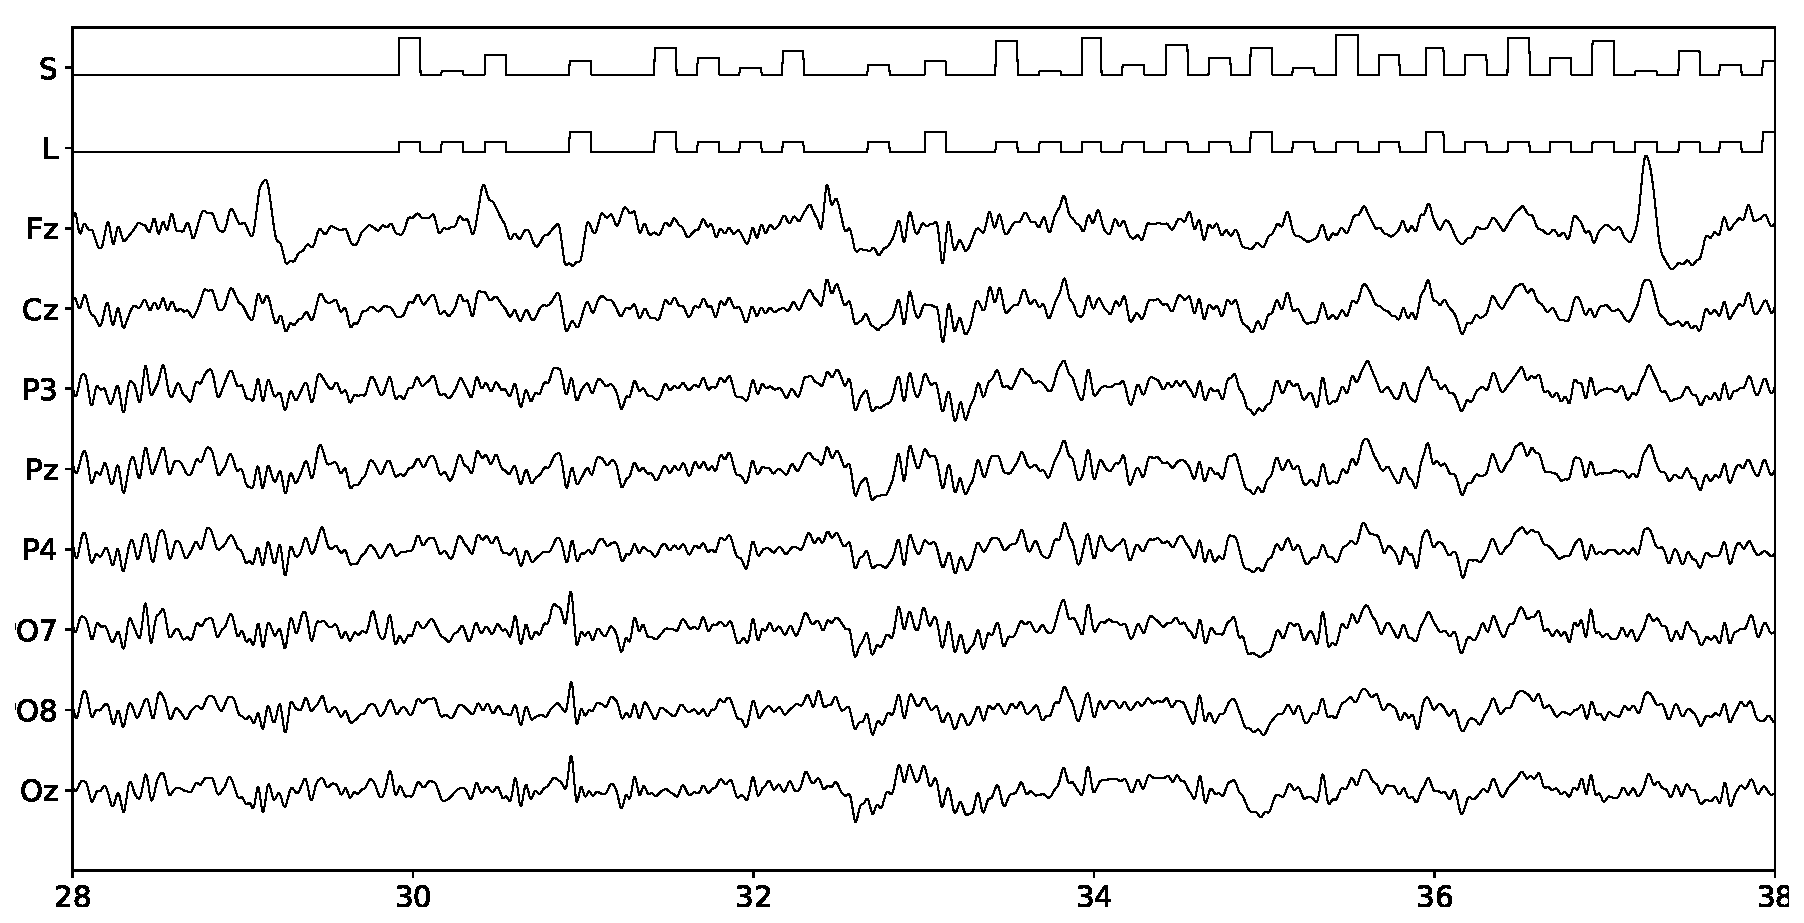
\includegraphics[width=.45\linewidth]{images/nogain.eps}}
\subfigure[The same eight-channel signal segment with the superimposed template.]{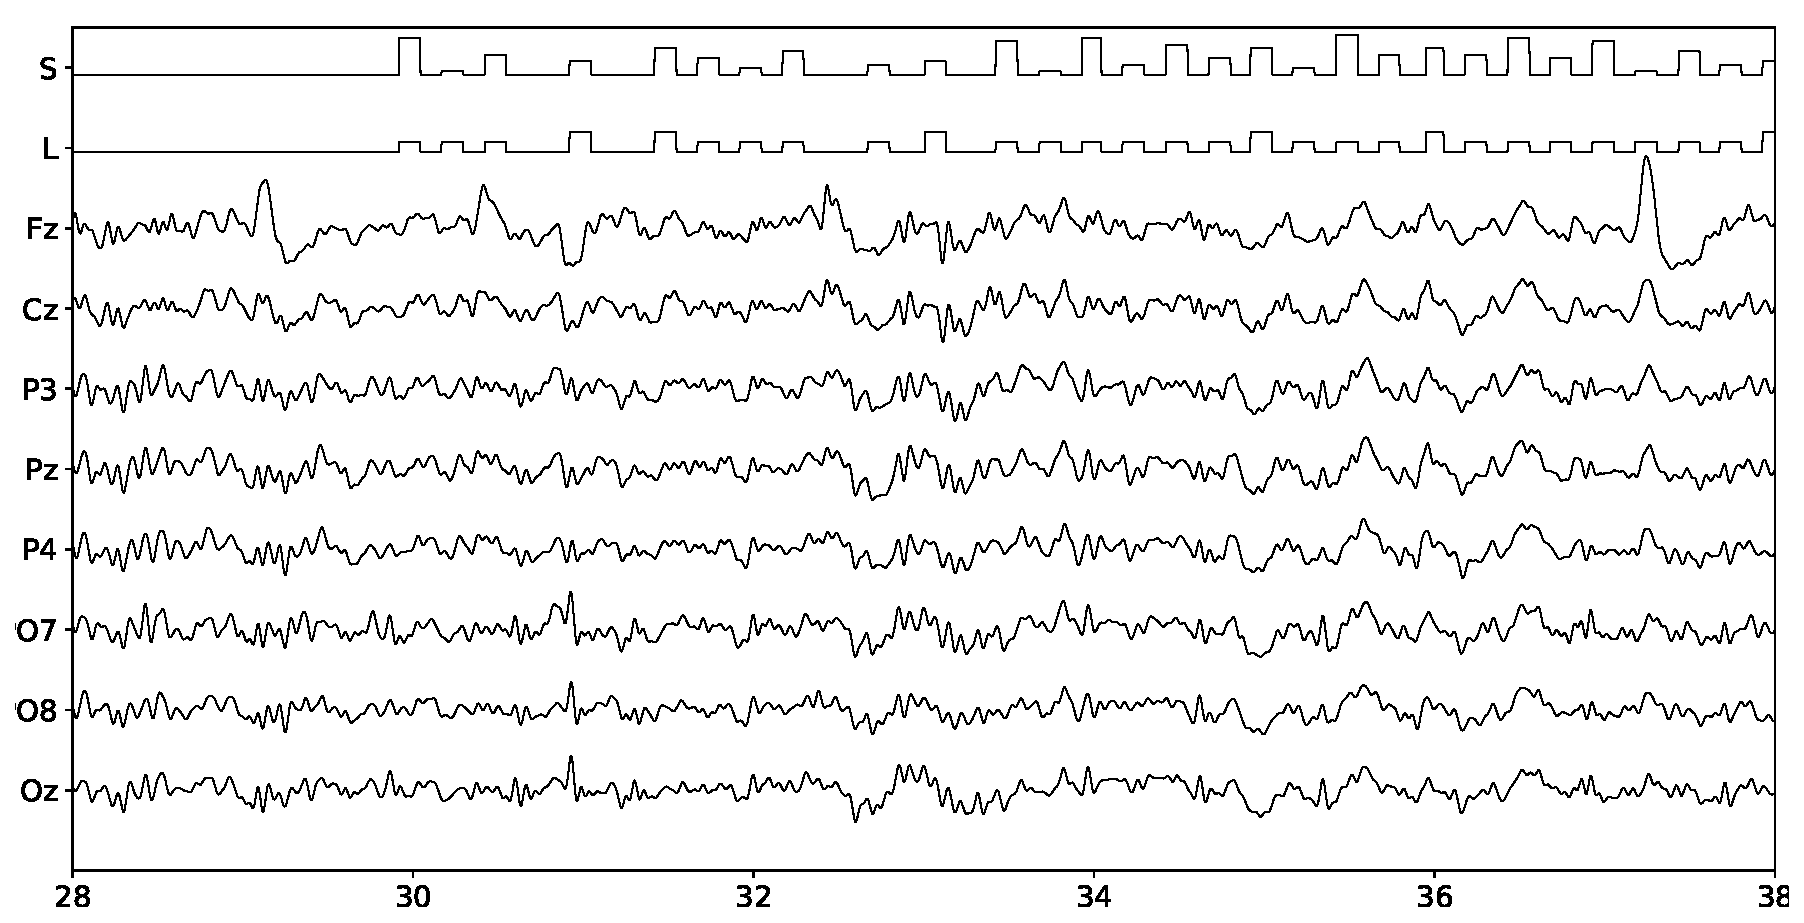
\includegraphics[width=.45\linewidth]{images/singlegain.eps}}
\subfigure[EEG sample of Cz and L channel of the original EEG trace.]{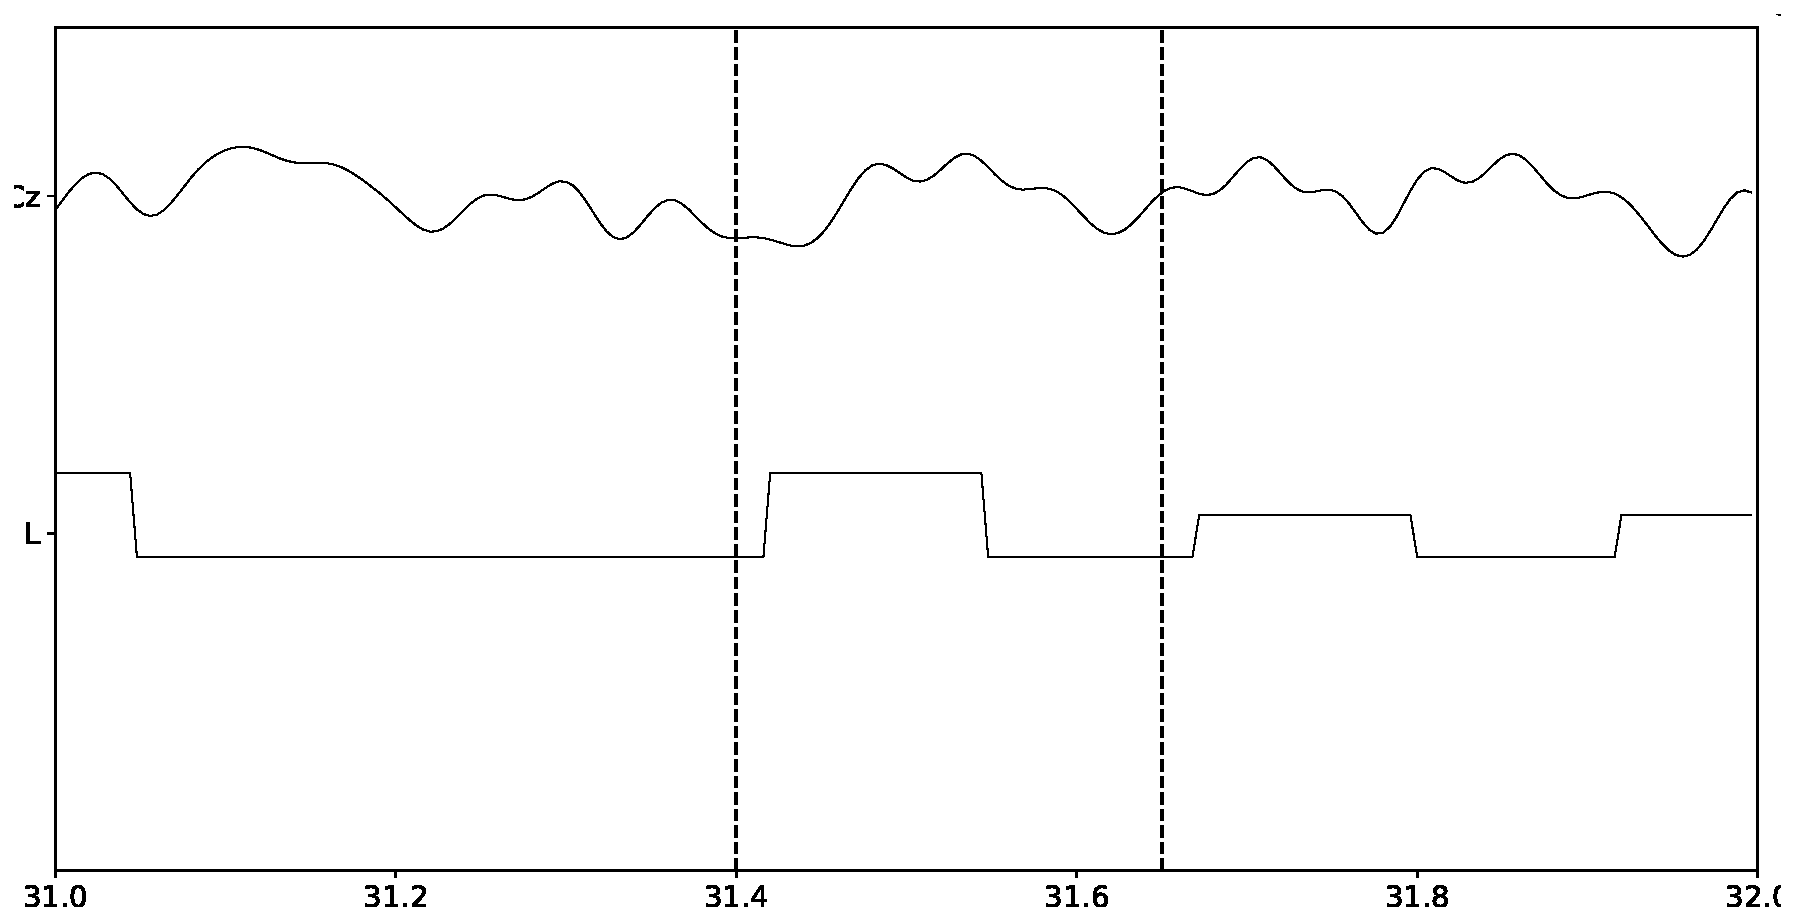
\includegraphics[width=.45\linewidth]{images/nogainzoomhit.eps}}
\subfigure[The same segment with the superimposed template.]{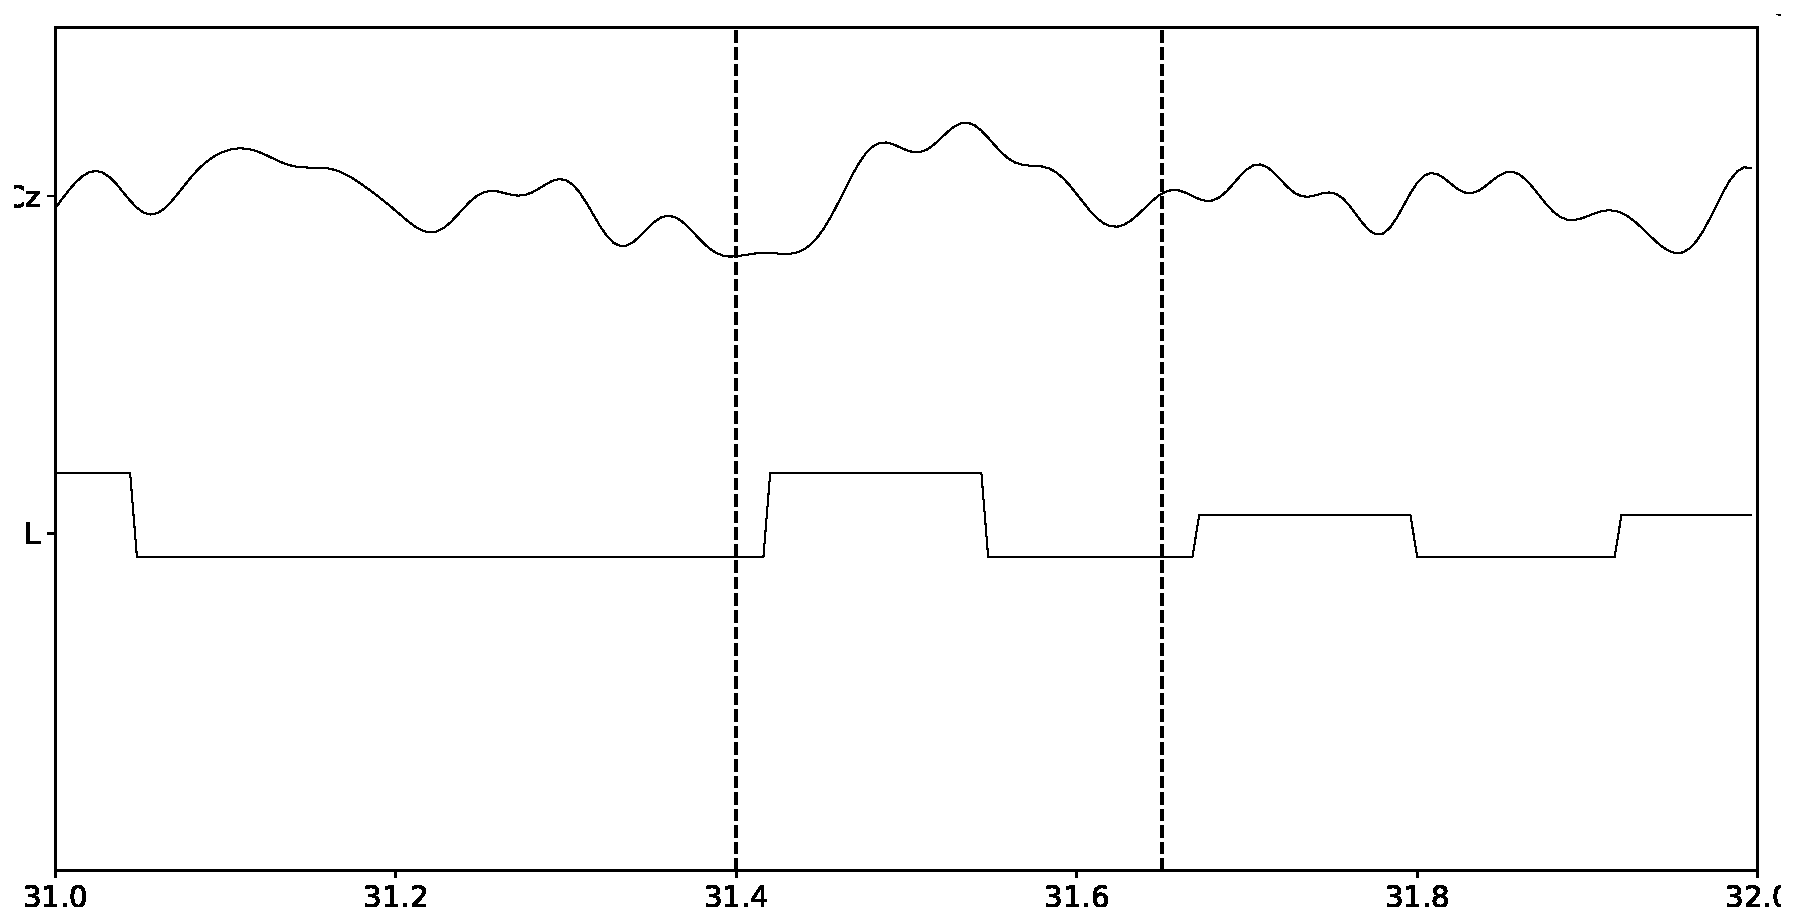
\includegraphics[width=.45\linewidth]{images/singlegainzoomhit.eps}}
\caption[Pseudo-real Dataset EEG Streams]{Eight-channel EEG signal without and with the superimposed ERP Template. The channel L, the mark which identifies where to superimpose the P300 ERP, is shown as well as the channel S which identifies the stimulus that was presented. On (c) and (d) the small variation that was introduced by the superimposition of the ERP can be seen enclosed by the vertical bars, where the slope of the bump on subfigure (d) is slightly bigger}
\label{fig:gains}
\end{figure}

Inter- and Intra-trial variability, with eventually cognitive implications, can alter the shape of the evoked P300 potential.  Hence, it is of interest to assess  at which extend waveform-based algorithm can handle these variations. Using this dataset, the following experiments are conducted to simulate known alterations over waveform components and to verify the performance of the algorithms expounded on Section~\ref{waveformalgorithms}, \textit{MP1}, \textit{MP2}, \textit{PE}, \textit{SHCC} and the one proposed by this Thesis: \textit{HIST}.

\begin{itemize}
\item Experiment 1 - Letter Identification Performance: the letter identification performance of each one of these methods on the artificially generated pseudo-real dataset.
\item Experiment 2 - Latency Noise:  Instead of superimposing the P300 ERP over the EEG trace at the exact locations where stimulus onsets are situated, an artificial latency lag is added.  The lagging value is picked from a uniform distribution $U(0,0.4)$ [s] ranging from $0$ to $0.4$ of the $1s$ segment size~\cite{DaPelo2018}.
\item Experiment 3 - Component Amplitude Noise: the amplitude of the main P3b component of the ERP template is randomly altered.  This component is defined to be located from the stimulus onset between $148$ ms up to $996$ ms which is around $840$ ms long.  This waveform element, multiplied by a gain factor, is subtracted from the original template.  This gain factor between $0$ and $1$ is drawn from a uniform distribution $U(0,1)$.  Additionally this subtracted waveform is multiplied by a Gaussian window with a support of the same length~\cite{Harris1978}.  This avoids adding any discontinuity into the artificial generated signal.
\end{itemize}


\begin{figure}[h!]
\centering
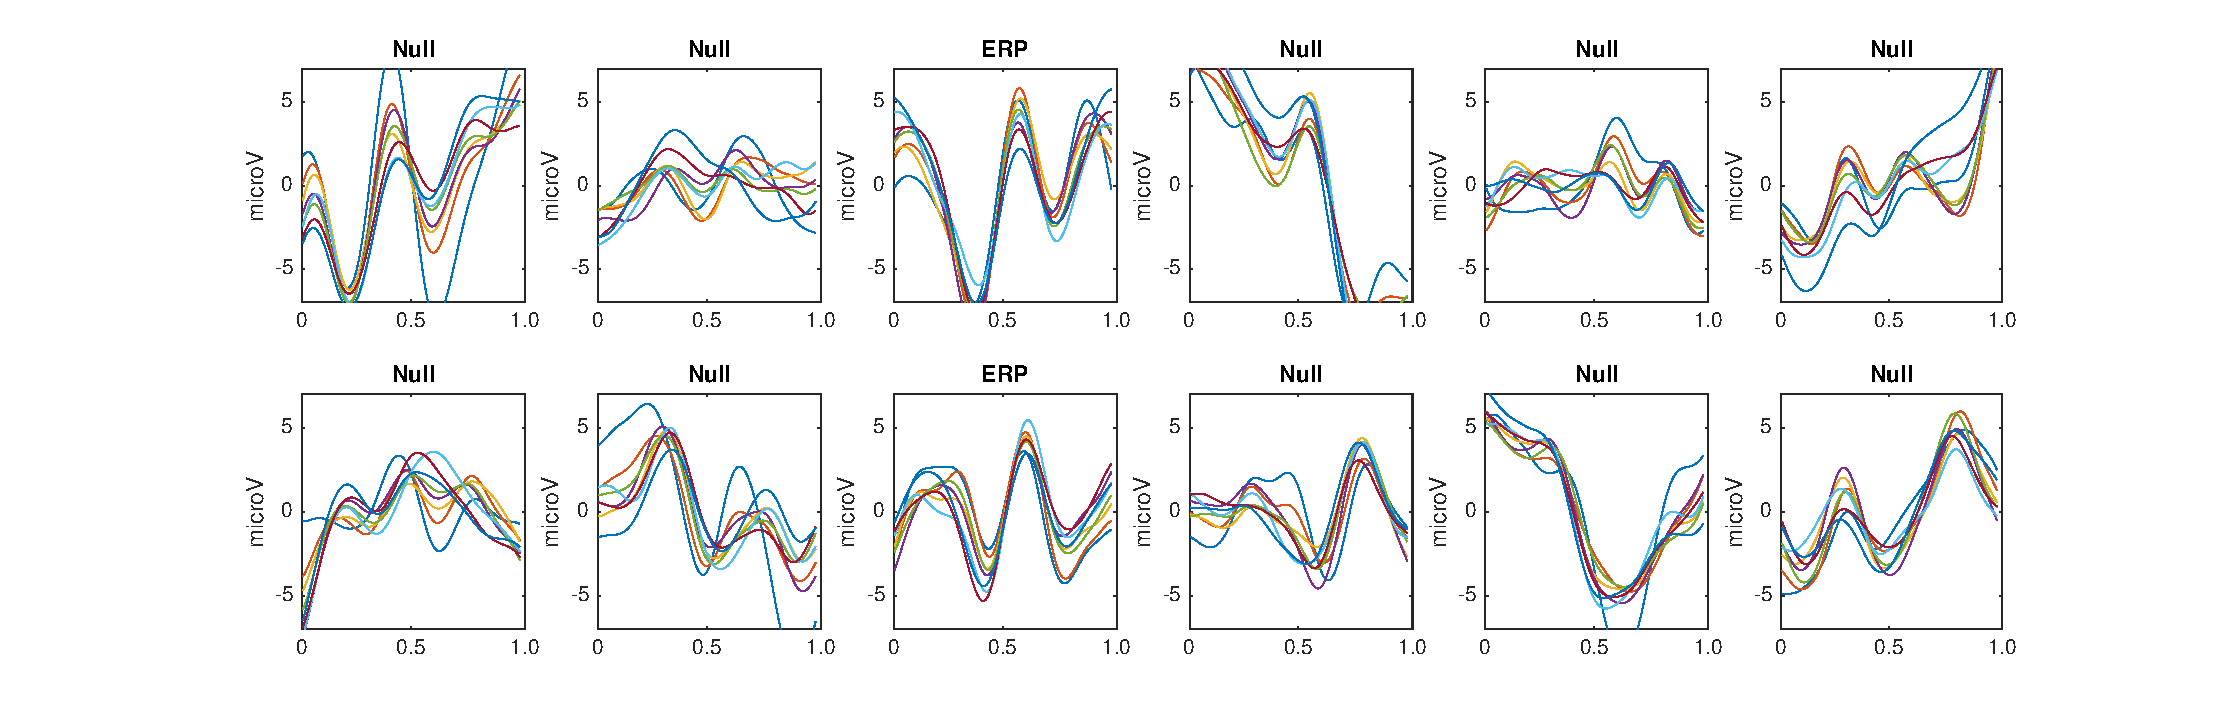
\includegraphics[width=1.0\linewidth]{images/GainCheck.eps}
\caption[P300 Averaged Segments for a single-intensification sequence]{Point-to-point averaged signals for the first letter identification trial.  The ERP is superimposed on locations 3 and 9.  Location $l=3$ is obtained while averaging the segments where the row of the speller matrix is intensified whereas locations 9 is calculated from the intensification of the corresponding column.}
\label{fig:gaincheck}
\end{figure}

The classification method Support Vector Machine \textit{SVM} with a linear kernel, is added for comparison as control using a feature $f$ constructed by normalizing the signal on each channel~\cite{Krusienski2006}.  This method has been proved efficient in decoding P300 in several BCI Competitions~\cite{Kaper2004}. 

All these experiments are executed using a cross-validation procedure dividing the letter to spell in two sets, preserving the structure of the letter identification trials. Spelling letters are scrambled while the order and group of each intensification sequence is preserved.

\subsubsection{Dataset IV - P300 Dataset IIb BCI Competition II (2003)}

Finally the performance at letter identifications for the method proposed on this Thesis and the other similar methods described in~\ref{waveformalgorithms} is evaluated by performing an offline BCI Simulation on the Dataset IIb of the BCI Competition II (2003)~\cite{Blankertz2002}.  The protocol of this dataset is very similar to what was used to obtain the pseudo-real dataset.  The sampling frequency of this dataset is $240$, the number of letters are $73$ where the first $42$ are used to create the template dictionary for all the methods and the remaining $31$ are used to test the character recognition rate performance.  Additionally, in this dataset the number of available intensification number sequences $\gls{ka}$ is $15$.  

%TODO Explicar este protocolo porque no es igual, de hecho es bastante distinto.

\subsubsection{Parameters}

The P300 event can have a span $\gls{lambda}$ of $400$ ms and its peak-to-peak amplitude $\gls{DeltamuV}$ can reach $ 10 \mu V $~\cite{Rao2013}.  Hence it is necessary to utilize a signal segment of size $\gls{w} = 1$ second.  In order to compute the patch parameters, Equations~\ref{eq:horizontalpatchscale} and \ref{eq:verticalpatchscale} are used to determine the value of $3$ for the horizontal patch scale $\gls{St}$ as well as the vertical patch scale $\gls{Sv}$.  It is important to remark that as it is described in Section~\ref{Pipeline} the effective sampling frequency $\gls{Fs}$ of the signal is $16\si{hertz}$.


%necesitamos definir el valor de s en función de los parámetros de la señal, de modo tal que el parche cubra el evento completo.  
%We propose the Equations~\ref{eq:mapping2} and~\ref{eq:mapping1} to compute the scale value in horizontal and vertical directions, respectively. 
%\begin{equation}
%s_x = \frac{ \gamma \;  \lambda \  F_s}{12}
%\label{eq:mapping2}
%\end{equation}
%
%\begin{equation}
%s_y= \frac{\gamma \; \Delta \mu V}{12} 
%\label{eq:mapping1}
%\end{equation}

As the peak-to-peak amplitude is small, to have a better resolution, the amplitude scales parameter are selected to be  $ \gamma = 4 $, and $\gls{gammat} = 4$.  With this configuration, the local patch and the descriptor can identify events of at most 16 $ \mu V $ of amplitude, with a span of $ \lambda = 0.99$ seconds, covering almost the entire segment.  According to Equations~\ref{eq:resolutiony} and \ref{eq:resolutionx}, this also determines that $ 1 $ pixel represents $ \frac{1}{\gamma}= \frac{1}{4} \mu V $ on the vertical direction, and $\frac{1}{\gls{Fs} \ \gls{gammat} }=\frac{1}{64}$ seconds on the horizontal direction. The keypoints  $\gls{kp}$  are located at $ (x_{k_p}, y_{k_p} )= ( 0.55 \gls{Fs} \ \gls{gammat}, z^l(c) )= (35,  z^l(c)) $ for the corresponding channel $c$ and location $l$ (see Equation~\ref{eq:zerolevel}).   In this way the whole transient event is captured. 

Lastly, the number of channels $C$ is equal to $8$ for the first three datasets and the number of intensification sequences $k_a$ is fixed to $10$.  The parameter $\gls{k}$ used to construct the set $N_T(\mathbf{q}^{(l,c)})$ is assigned to $k=7$, which was found empirically to achieve better results.  In addition, the norm used on  Equations \ref{eq:multiclassificationrow} and \ref{eq:multiclassificationcol} is the cosine norm, and descriptors are normalized to $ \left[ -1, 1 \right] $ (check Chapter~\ref{chapter:eleven}).

\section{Results}

Table~\ref{tab:resultsals} shows the results of applying the Histogram of Gradient Orientations (HIST) algorithm to the subjects of the public dataset of ALS patients. The percentage of correctly spelled letters is calculated while performing an offline BCI Simulation.  From the seven words for each subject, the first three are used for calibration, and the remaining four are used for testing.  The best performing channel  $\gls{bpc}$ is informed as well. The target ratio is $1:36$; hence theoretical chance level is $2.8\%$. It can be observed that the best performance of the letter identification method is reached in a dissimilar channel depending on the subject being studied.  Table~\ref{tab:resultsals} and~\ref{tab:resultsown} show for comparison the obtained performance rates using single-channel signals with the Support Vector Machine (SVM) classifier.  This method is configured to use a linear kernel.  The best performing channel $\gls{bpc}$, where the best letter identification rate was achieved, is also depicted.


\begin{table}[h!]
\caption[Dataset I - Single Channel Character Recognition Rates]{Dataset I: Character recognition rates for the public dataset of ALS patients using the Histogram of Gradient (HIST) calculated from  single-channel plots.  Performance rates using single-channel signals with the SVM classifier are shown for comparison.  The best performing channel $bpc$ for each method is visualized}
\centering
%% \tablesize{} %% You can specify the fontsize here, e.g.  \tablesize{\footnotesize}. If commented out \small will be used.
\begin{tabular}{c|cc|cc}
\toprule
\textbf{Participant}	&  $bpc$ 	&  HIST &  $bpc$	&  Single Channel SVM \\
\midrule
1     &     Cz   &   $35\%$    &  Cz   & $15\%$   \\
2     &     Fz   &   $85\%$      &  PO8   & $25\%$   \\
3     &     Cz   &   $25\%$    &  Fz   & $5\%$   \\
4     &     PO8 &   $55\%$   &  Oz   & $5\%$    \\
5     &     PO7 &   $40\%$    &  P3   & $25\%$   \\
6     &     PO7 &   $60\%$  &  PO8   & $20\%$    \\
7     &     PO8 &   $80\%$   &  Fz   & $30\%$     \\
8     &     PO7 &   $95\%$     &  PO7   & $85\%$ \\

%\bottomrule
\end{tabular}
\label{tab:resultsals}
\end{table}

%The spelled words are \textit{MANSO},\textit{CINCO},\textit{JUEGO} and \textit{QUESO}.

\begin{table}[h!]
\caption[Dataset II - Single Channel Character Recognition Rates]{Dataset II: Character recognition rates and $bpc$  using HIST calculated from  single-channel signals.  Performance rates using single-channel signals with the SVM classifier are shown for comparison.}
\centering
%% \tablesize{} %% You can specify the fontsize here, e.g.  \tablesize{\footnotesize}. If commented out \small will be used.
\begin{tabular}{c|cc|cc}
\toprule
\textbf{Participant}	&  $bpc$	&  HIST &  $bpc$	&  Single Channel SVM \\
\midrule
1     &     Oz   &   $40\%$  &  Cz   &  $10\%$    \\
2     &     PO7   &   $30\%$      &  Cz   & $5\%$   \\
3     &     P4   &   $40\%$    &  P3   & $10\%$    \\
4     &     P4 &   $45\%$    &  P4   & $35\%$     \\
5     &     P4 &   $60\%$  &  P3   & $10\%$     \\
6     &     Pz &   $50\%$ &  P4   & $25\%$     \\
7     &     PO7 &   $70\%$  &  P3   & $30\%$     \\
8     &     P4 &   $50\%$    &  PO7   & $10\%$    \\

%\bottomrule
\end{tabular}
\label{tab:resultsown}
\end{table}

% Agregar la clasificacion perfecta en base a que no considerabamos la varianza de la senial graficada

%The spelled words are \textit{GATTO}, \textit{MENTE}, \textit{VIOLA} and \textit{REBUS}.

The Information Transfer Rate (ITR), or Bit Transfer Rate (BTR), in the case of reactive BCIs~\cite{WolpawJonathanR2012}  depends on the amount of signal averaging required to transmit a valid and robust selection.  Figure~\ref{fig:performance} shows the performance curves for varying intensification sequences for the subjects included in the dataset of ALS patients. It can be noticed that the percentage of correctly identified letters depends on the number of intensification sequences that are used to obtain the averaged signal.  Moreover, when the number of intensification sequences tend to 1, which corresponds to single-intensification character recognition, the performance is reduced. As mentioned before, the SNR of the P300 obtained from only one segment of the intensification sequence is very low and the shape of its P300 component is not very well defined.



\begin{figure}[h!]
\centering
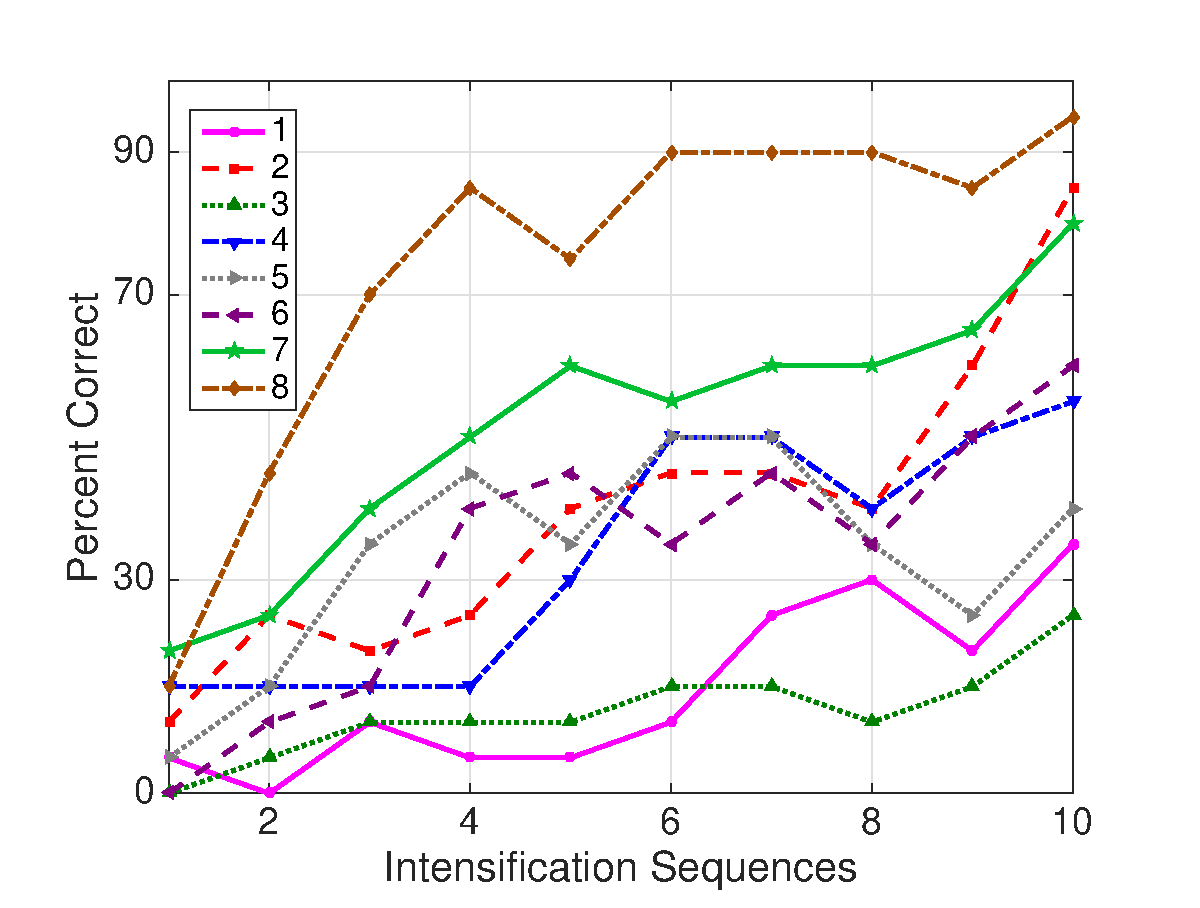
\includegraphics[width=10cm]{images/performance.eps}
\caption[Dataset I ALS Patients Dataset P300 Performance Curves]{Performance curves for the eight subjects included in the dataset I of ALS patients.  Three out of eight subjects achieved the necessary performance to implement a valid P300 speller.}
\label{fig:performance}
\end{figure}




In Table~\ref{tab:resultsown} the results obtained for 8 healthy subjects are shown.  It can be observed that the performance is above chance level. It was verified that HIST method has an improved performance at letter identification than SVM that process the signals on a channel by channel strategy (Wilcoxon signed-rank test, $p =  0.004$ for both datasets).


\begin{table}[h!]
\caption[Dataset I - Comparisons of Character Recognition Rates]{Character recognition rates and the best performing channel $bpc$ for the public dataset I  using the HIST versus performance rates obtained by SWLDA and SVM classification algorithms with a multichannel concatenated feature.}
\centering
%% \tablesize{} %% You can specify the fontsize here, e.g.  \tablesize{\footnotesize}. If commented out \small will be used.
\begin{tabular}{c|cc|c|c}
\toprule
%\textbf{Participant}	&  \textbf{BPC}	& \multicolumn{2}{c}{Character Recognition Rates}\\
%\cline{1-5} \\
\textbf{Participant}	&  $bpc$	&  HIST & Multichannel SWLDA & Multichannel SVM \\
                                    &  for HIST        &           &                                       &   \\
\midrule
1     &     Cz   &   $35\%$  & $45\%$  & $40\%$\\
2     &     Fz   &   $85\%$  & $30\%$   & $50\%$   \\
3     &     Cz   &   $25\%$  & $65\%$ & $55\%$   \\
4     &     PO8 &   $55\%$ & $40\%$  & $50\%$   \\
5     &     PO7 &   $40\%$ & $35\%$  & $45\%$   \\
6     &     PO7 &   $60\%$ &  $35\%$  & $70\%$   \\
7     &     PO8 &   $80\%$ & $60\%$   & $35\%$   \\
8     &     PO7 &   $95\%$  & $90\%$   & $95\%$  \\

%\bottomrule
\end{tabular}
\label{tab:resultsalsswlda}
\end{table}

%In Tables~\ref{tab:resultsals} and~\ref{tab:resultsown} results for character recognition rates using single channel signals with the SVM~\cite{Scholkopf2001}  classification algorithm are also shown.    This algorithm was configured to use a linear kernel.  The best performing channel where the best letter identification rate was obtained is also depicted.

%The PE algorithm, which is also devised on a time-domain description of the waveform, was implemented according to \cite{Unakafova2013} and its parameters were adjusted as stated by \cite{Zanin2012}, with an \textit{order} of $2$ and a \textit{sliding window} of size $10$. 

Tables~\ref{tab:resultsalsswlda} and~\ref{tab:resultsownswlda} are presented in order to compare the performance of the HIST method versus a multichannel version of the SWLDA and SVM classification algorithms for both datasets.  The feature was formed by concatenating all the channels~\cite{Krusienski2006}.  SWLDA is the methodology proposed by the ALS dataset's publisher.  As can be observed in Figure~\ref{fig:boxplots}, It was verified for the dataset I of ALS patients that it has similar performance  against other methods like SWLDA or SVM, which use a multichannel feature (Quade test with $p=0.55$) whereas for the dataset of healthy subjects significant differences were found (Quade test with $p=0.02$) where only the HIST method achieved a different performance than SVM (with multiple comparisons, significant difference of level $0.05$).

\begin{figure}[h!]
\centering
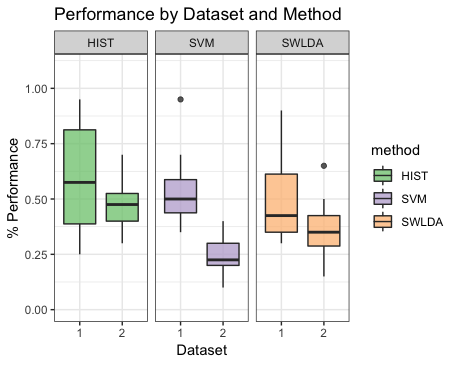
\includegraphics[width=10cm]{images/boxplots.png}
\caption[Dataset I and II Performances Boxplots]{Boxplots obtained for the methods HIST and multichannel SVM and SWLDA for the Datsets I and II.  The achieved performance for the HIST method is similar to the performace obtained for the other methods (Quade test with $p=0.55$).}
\label{fig:boxplots}
\end{figure}

\begin{table}[h!]
\caption[Dataset II - Comparisons of Character Recognition Rates]{Character recognition rates and the best performing channel $bpc$ for the  dataset II  using the HIST versus performance rates obtained by SWLDA and SVM classification algorithms with a multichannel concatenated feature.}
\centering
%% \tablesize{} %% You can specify the fontsize here, e.g.  \tablesize{\footnotesize}. If commented out \small will be used.
\begin{tabular}{c|cc|c|c}
\toprule
%\textbf{Participant}	&  \textbf{BPC}	& \multicolumn{2}{c}{Character Recognition Rates}\\
%\cline{1-5} \\
\textbf{Participant}	&  $bpc$ 	&  HIST & Multichannel SWLDA & Multichannel SVM  \\
                                    &  for HIST        &           &                                       &   \\
\midrule
1     &     Oz   &     $40\%$  &     $65\%$  &     $40\%$ \\
2     &     PO7   &     $30\%$ &   $15\%$  &     $10\%$ \\
3     &     P4   &     $40\%$ &     $50\%$  &     $25\%$ \\
4     &     P4   &     $45\%$ &     $40\%$  &     $20\%$ \\
5     &     P4   &      $60\%$ &    $30\%$  &     $20\%$ \\
6     &     Pz   &      $50\%$ &    $35\%$  &     $30\%$ \\
7     &     PO7   &      $70\%$ &  $25\%$  &     $30\%$ \\
8     &     P4   &      $50\%$ &    $35\%$  &     $20\%$ \\

%\bottomrule
\end{tabular}
\label{tab:resultsownswlda}
\end{table}

%It was verified for the dataset of ALS patients that it has similar performance  against other methods like SWLDA or SVM, which use a multichannel feature (Quade test with $p=0.55$) whereas for the dataset of healthy subjects significant differences where found (Quade test with $p=0.02$) where the HIST method achieved a better performance than SVM (with multiple comparisons, significant difference of level $0.05$).
 
%\subsection{Occipital Channels}

The P300 ERP  consists of two overlapping components: the P3a and P3b, the former with frontocentral distribution while the later stronger on centroparietal region~\cite{Polich2007}. Hence, it is known that the stronger response of this ERP is usually found on the central channel Cz~\cite{Riccio2013}. However, \cite{Krusienski2006} shows that the response may also arise in occipital regions.  We found that by analyzing only the waveforms, occipital channels PO8 and PO7 show higher performances for some subjects. 

%\subsection{Stability of the P300 shape}

As subjects have varying \textit{latencies} and \textit{amplitudes} of their P300 components, they also have a varying stability of the \textit{shape} of the generated ERP \cite{Nam2010}.  Figure~\ref{fig:p300templates} shows 10 sample P300 templates patches for patients 8 and 3 from the dataset of ALS patients. It can be discerned that in coincidence with the performance results, the P300 signature is more clear and consistent for subject 8 (A) while for subject 3 (B) the characteristic pattern is more difficult to perceive.


\begin{figure}[h!]
\centering
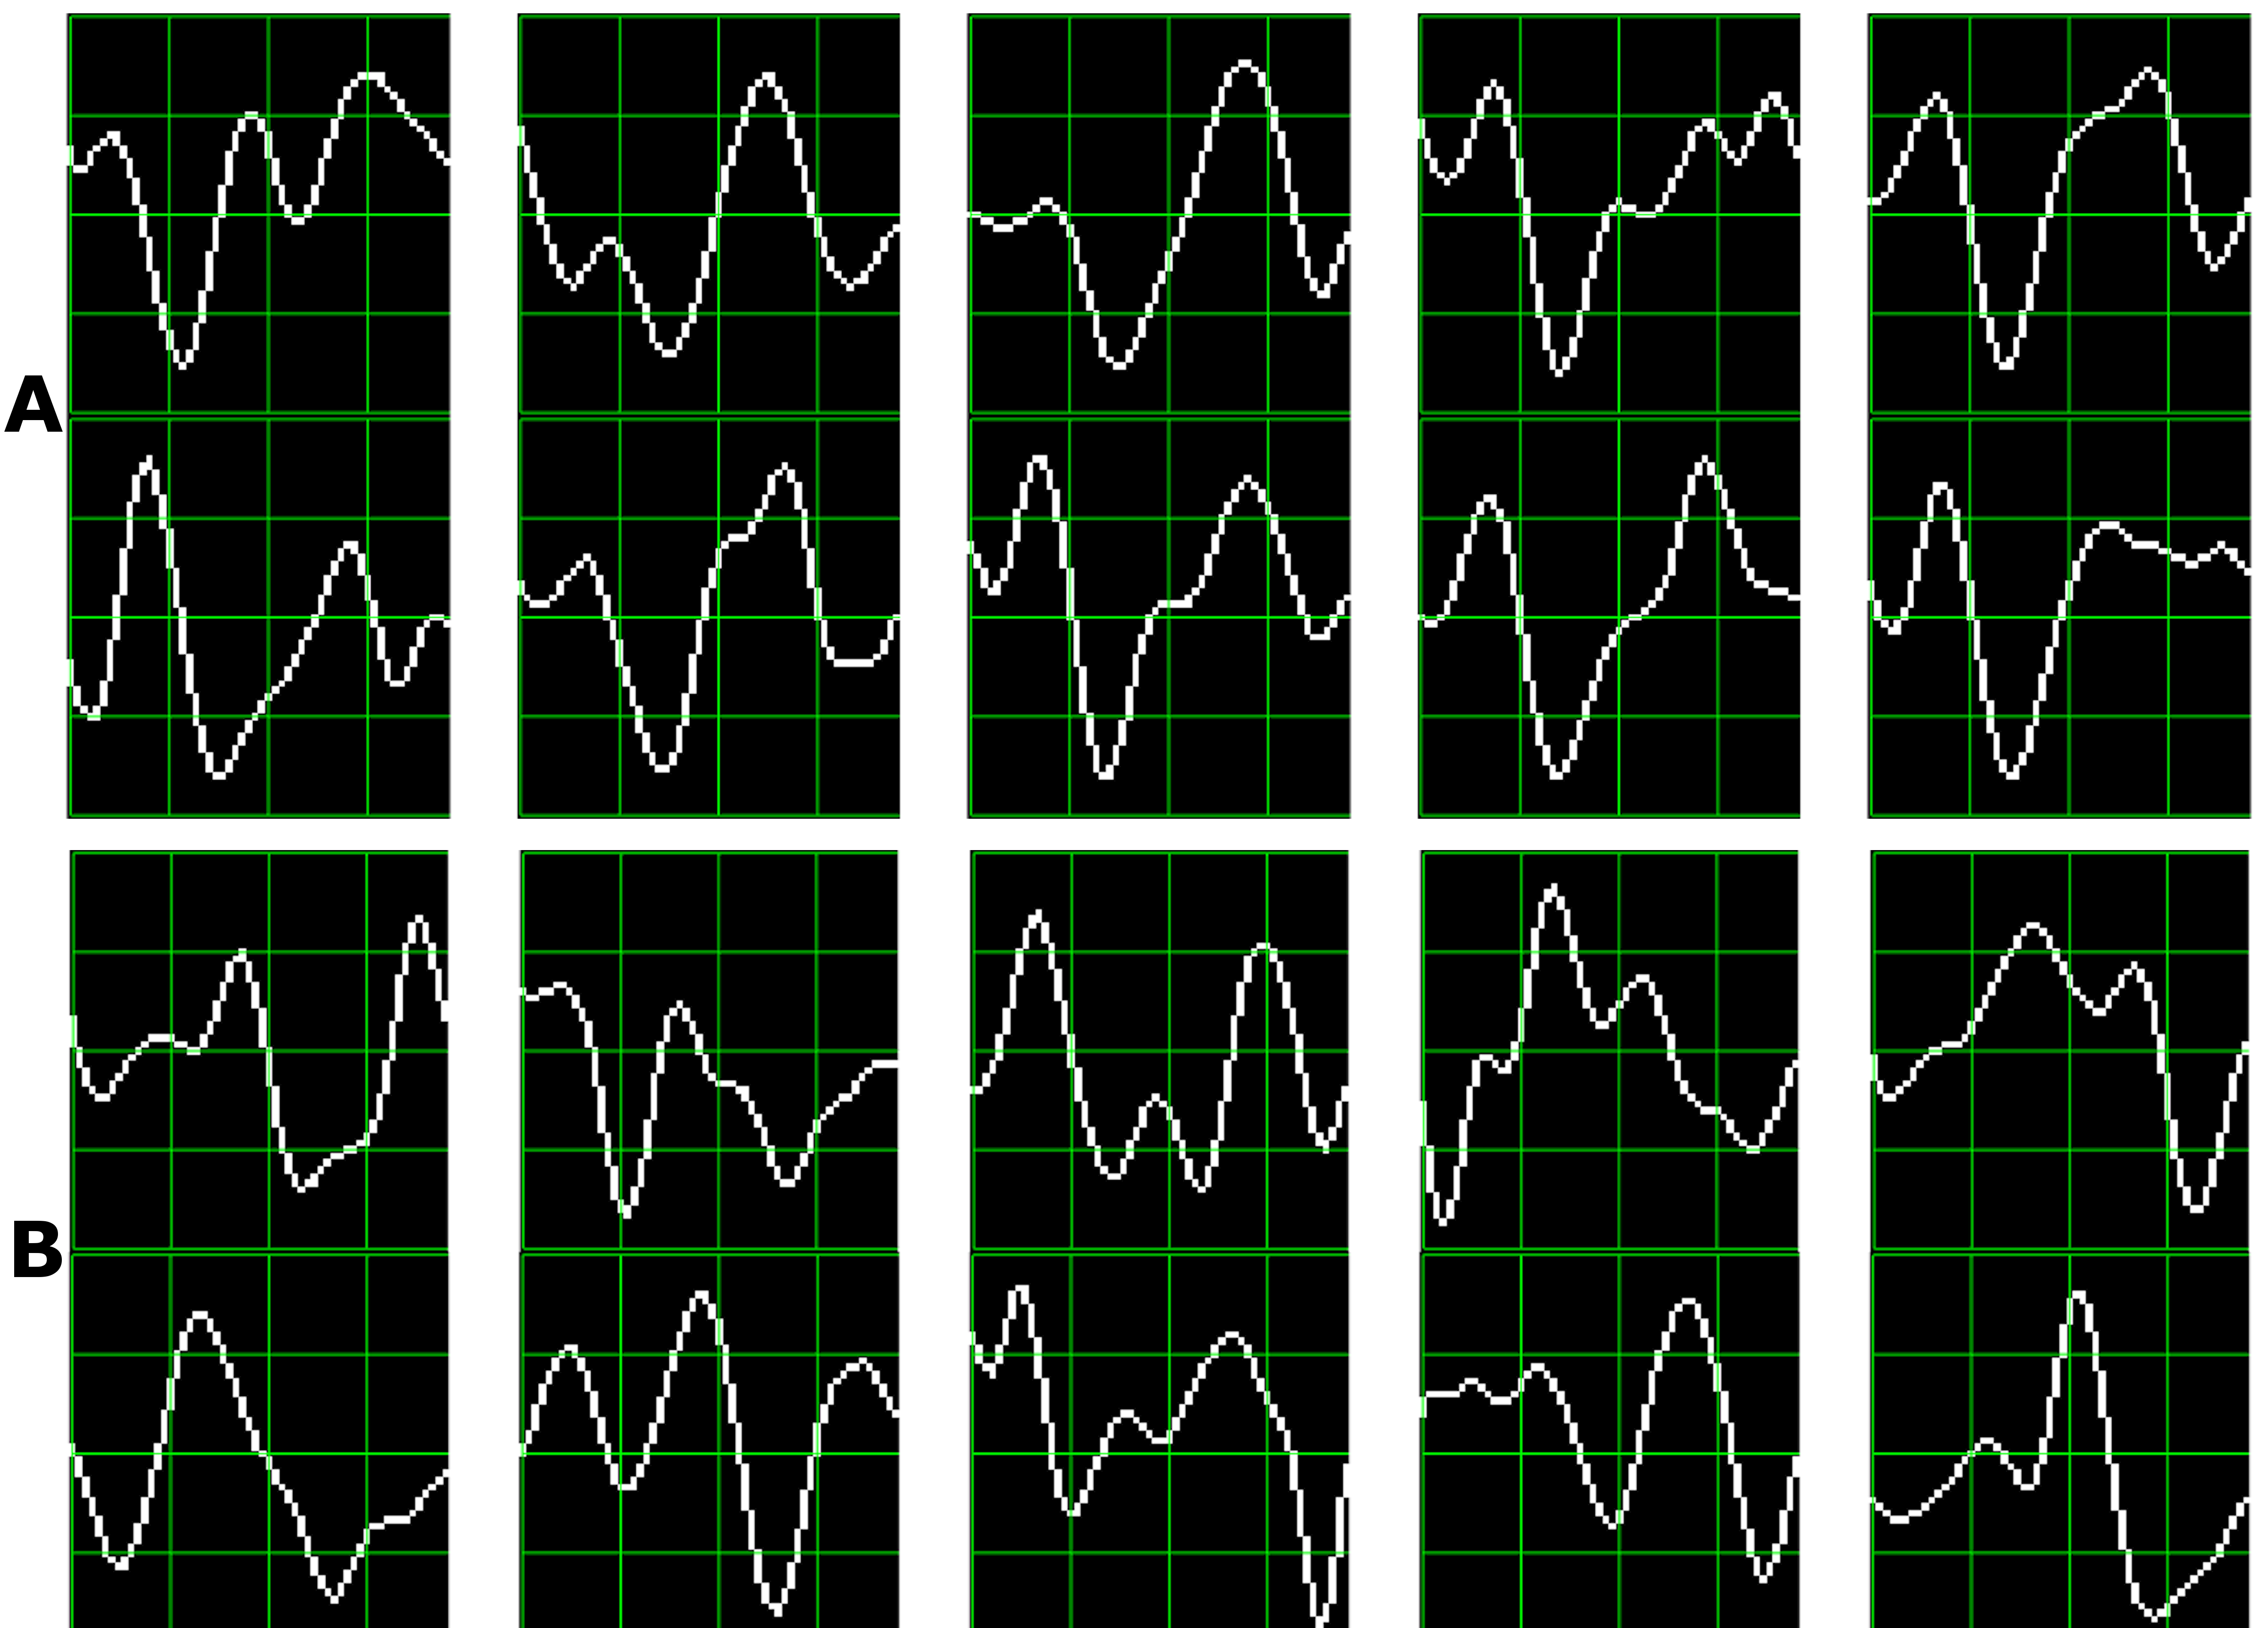
\includegraphics[width=15cm]{images/subject.png}\label{subject8}
\caption[Sample P300 Patches]{Ten sample P300 template patches for subjects 8 (A) and 3 (B) of the public Dataset I of ALS patients.  Downward deflection is positive polarity. }
\label{fig:p300templates}
\end{figure}


Additionally, the stability of the P300 component waveform has been extensively studied in patients with ALS \cite{SellersandEmanuelDonchin2006,TomohiroMadarame2008,Nijboer2009,Mak2012,McCane2015} where it was found that these patients have a stable P300 component, which were also sustained across different sessions.  In line with these results we do not find evidence of a difference in terms of the performance obtained by analyzing the waveforms (HIST) for the group of patients with ALS and the healthy group of volunteers (Mann-Whitney U Test, $p=0.46$). Particularly, the best performance is obtained for a subject from the ALS dataset for which, based on visual observation, the shape of they P300 component is consistently identified.

%\subsection{Descriptor Space and classification method}

It is important to remark that when applied to binary images obtained from signal plots, the feature extraction method described in Section \ref{SIFT} generates sparse descriptors.  Under this subspace we found that using the cosine metric yielded a significant performance improvement (check Chapter~\ref{chapter:eleven}). On the other hand, the unary classification scheme based on the NBNN algorithm proved very beneficial for the P300 Speller Matrix.  This is due to the fact that this approach solves the unbalance dataset problem which is inherent to the oddball paradigm~\cite{Tibon2015}.  

%Using the same feature but with classification methods SVM, feed forward Neural Networks and SWLDA  common in BCI Research achieved a reduced performance.


Regarding Experiments 1,2 and 3 for the Dataset III, results are shown in Table~\ref{tab:results} and in Figure~\ref{fig:performancetest}, ~\ref{fig:performancetestlatency} and~\ref{fig:performancetestamplitude}.  Table~\ref{tab:results} shows the  performance while identifying each letter of the standard P300 Speller Matrix, and the $\gls{bpc}$, the channel where the best performance is attained.   Figure~\ref{fig:performancetest} shows the performance curves for the six algorithms under comparison.  Each one represents the percentage of letters that is actually predicted by each algorithm using a cross-validation procedure.  As previously described the data is continuously divided in two sets, where the first 15 letters are used to derive the dictionary of templates while the remaining 20 letters are used to measure the letter identification performance. This is repeated one hundred times, and performances averaged.   Figure~\ref{fig:performancetestlatency} shows the same results for the Experiment 2, where a noisy latency lag was included.   Lastly, Figure ~\ref{fig:performancetestamplitude} represents the performance values obtained for the Experiment 3, when the amplitude of the P3b component of the template is randomly attenuated.  

\begin{figure}[h!]
\centering
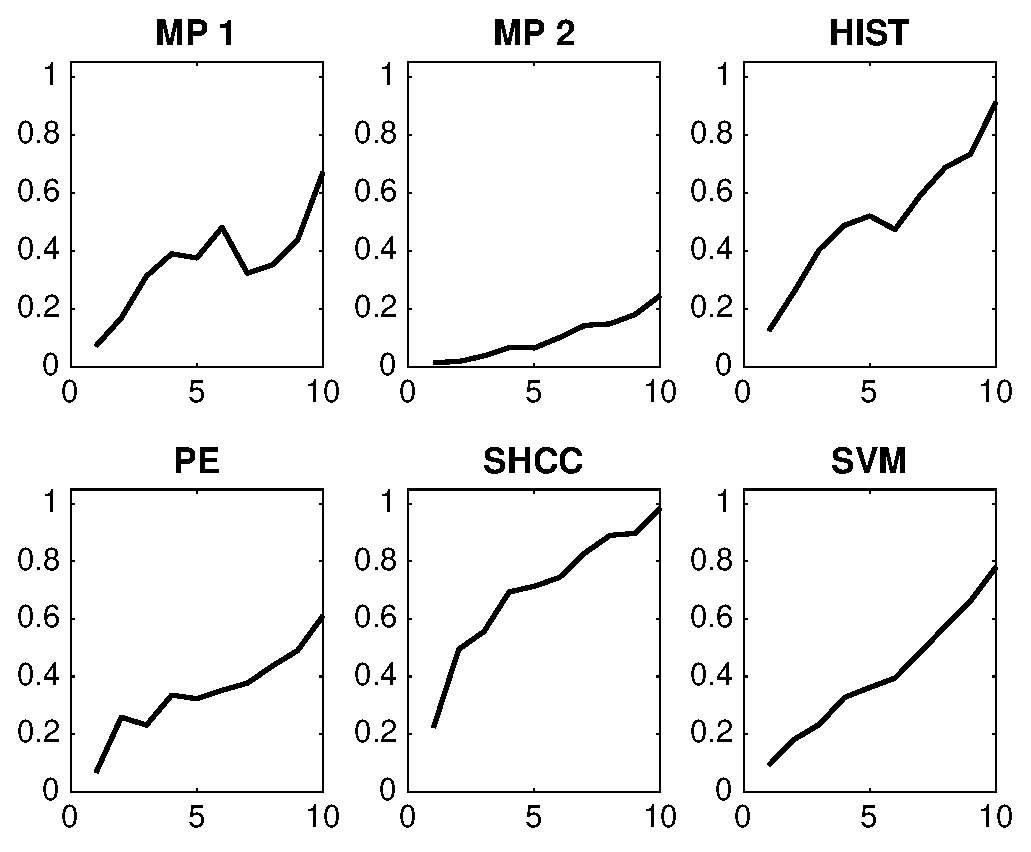
\includegraphics[width=15cm]{images/CrossPerformanceTest.eps}
\caption[Experiment I Pseudo-real Dataset III Speller Performance]{Speller performance obtained for each method for the Experiment 1.  Y-axis shows performance accuracy while X-axis shows the number of intensification sequences used to calculate the point-to-point signal average.}
\label{fig:performancetest}
\end{figure}

\begin{figure}[h!]
\centering
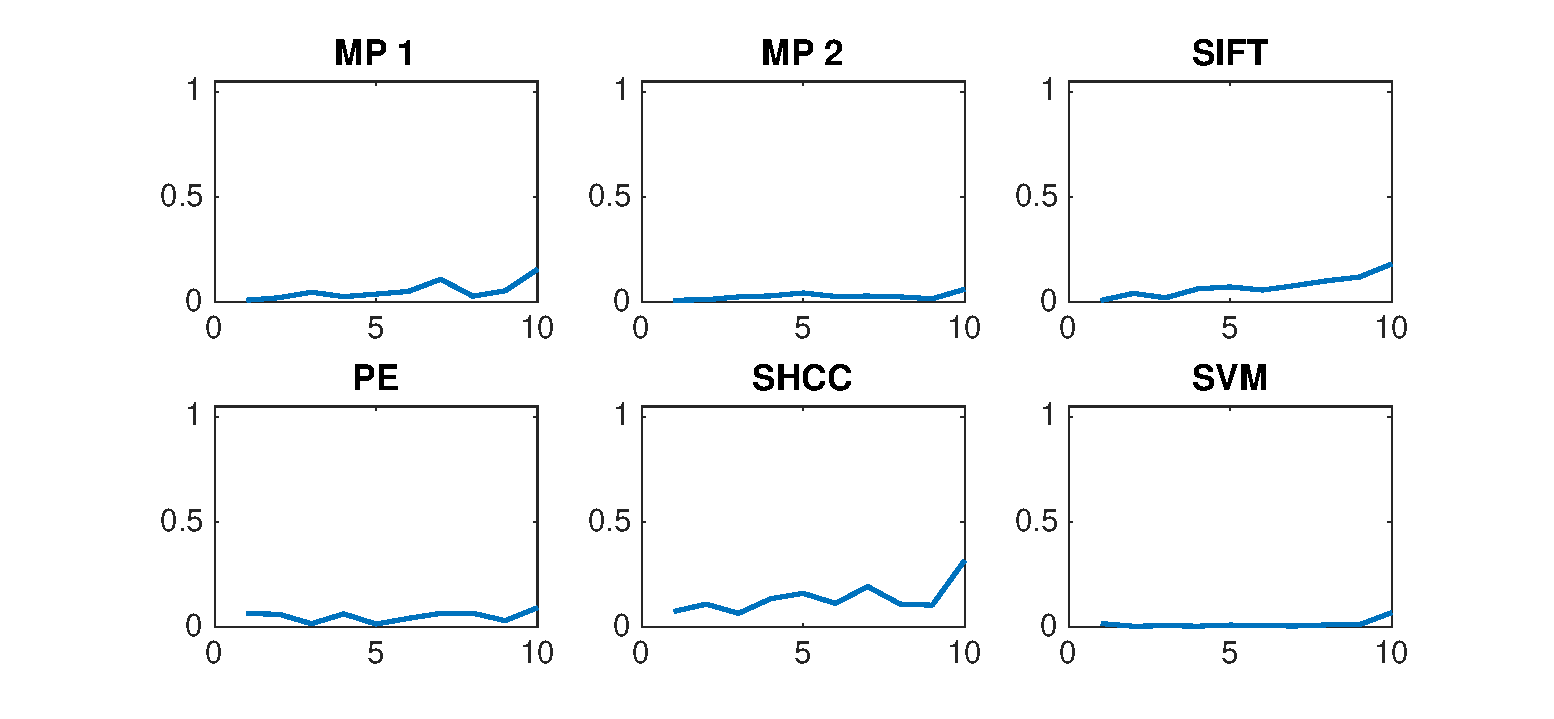
\includegraphics[width=15cm]{images/CrossPerformanceTestLatency.eps}
\caption[Experiment II Pseudo-real Dataset III Speller Performance]{Speller performance obtained for each method while latencies are artificially added to each single-intensification segment corresponding to the Experiment 2.  The achieved performance is significantly reduced for all methods. Y-axis shows letter identification performance while X-axis shows the number of intensification sequences used to calculate the ensemble average.}
\label{fig:performancetestlatency}
\end{figure}

\begin{figure}[h!]
\centering
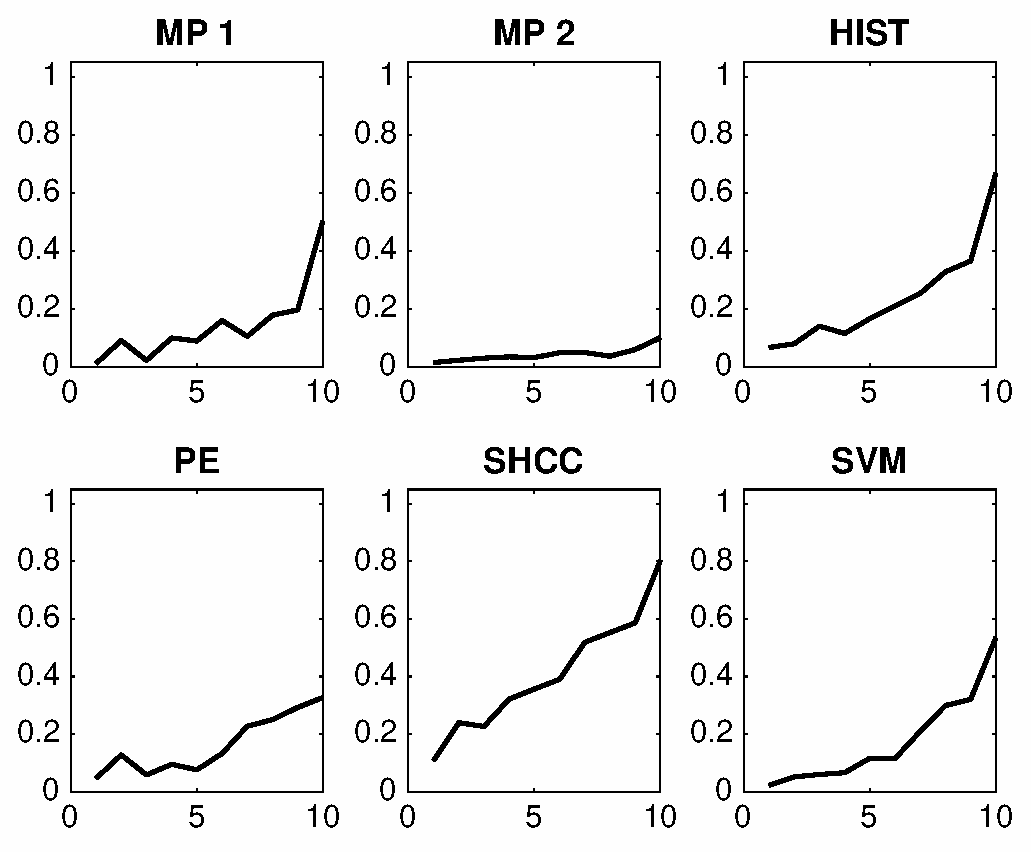
\includegraphics[width=15cm]{images/CrossPerformanceTestAmplitude.eps}
\caption[Experiment III Pseudo-real Dataset III Speller Performance]{Speller performance obtained for the Experiment 3 while the amplitudes of the P3b component of the superimposed ERP is randomly reduced. Y-axis shows performance accuracy while X-axis shows the number of intensification sequences.}
\label{fig:performancetestamplitude}
\end{figure}

\begin{table}[h!]
\caption[Pseudo-real Dataset Speller Performance]{Speller classification performance obtained for all the waveform-based algorithms: MP Matching Pursuit, SIFT Scale Invariant Feature Transform, PE Permutation Entropy and SHCC Slope Horizontal Code Chain. Additionally, the control algorithm SVM Support Vector Machines is included for comparison.  All the methods process the signal on a channel-by-channel basis, hence the best performing channel is also shown. In this case with absence of null-signals, it can be interpreted as the channel that adds less noise to the ERP template.  All the methods used $10$ intensification sequences to coherently average the trials to obtain the averaged signal. }
\centering
%% \tablesize{} %% You can specify the fontsize here, e.g.  \tablesize{\footnotesize}. If commented out \small will be used.
\begin{tabular}{ccccc}
\toprule
\textbf{Method}	& \textbf{Channel} &   \multicolumn{3}{c}{Performance} \\
%\cline{3-5} \\
 	&  &  \textbf{Experiment 1} & \textbf{Experiment 2}	& \textbf{Experiment 3}\\
\midrule
MP 1 & PO8  & $67\%$ & $15\%$ & $50\%$\\
MP 2 & PO7 & $24\%$ & $6\%$ & $10\%$\\
SIFT  & PO8 & $91\%$ & $18\%$ & $66\%$\\
PE     & Cz & $61\%$ & $9\%$ & $32\%$\\
SHCC & P4 & $98\%$ & $31\%$ & $80\%$\\
SVM     & PO8  & $78\%$ & $7\%$ & $53\%$\\
\bottomrule
\end{tabular}
\label{tab:results}
\end{table}

Finally, results obtained for the dataset BCI Competition 2003 IIb are shown in Figures \ref{fig:performancebcicompetition} and in Table~\ref{tab:bcicompetitionresults}.  For this experiment the number of available intensification sequences is 15.

\begin{table}[h!]
\caption[Dataset IIb BCI Competition II (2003) Speller Performance]{Speller classification performance obtained for the dataset IIb of the BCI Competition II (2003) for each one of the algorithms using $15$ repetitions of intensification sequences. The first $42$ trials are used for training to build the template dictionary and the remaining $31$ for testing. The channel where the best performance is attained, is also shown. }
\centering
%% \tablesize{} %% You can specify the fontsize here, e.g.  \tablesize{\footnotesize}. If commented out \small will be used.
\begin{tabular}{ccc}
\toprule
\textbf{Method}	& \textbf{Channel} &  \textbf{Performance} \\
\midrule
MP 1 & FC2  & $50\%$ \\
MP 2 & CPz & $22\%$ \\
SIFT  & Cz & $67\%$ \\
PE     & PO8 & $22\%$ \\
SHCC & Cz & $61\%$ \\
SVM     & C1  & $32\%$ \\
\bottomrule
\end{tabular}
\label{tab:bcicompetitionresults}
\end{table}

\begin{figure}[h!]
\centering
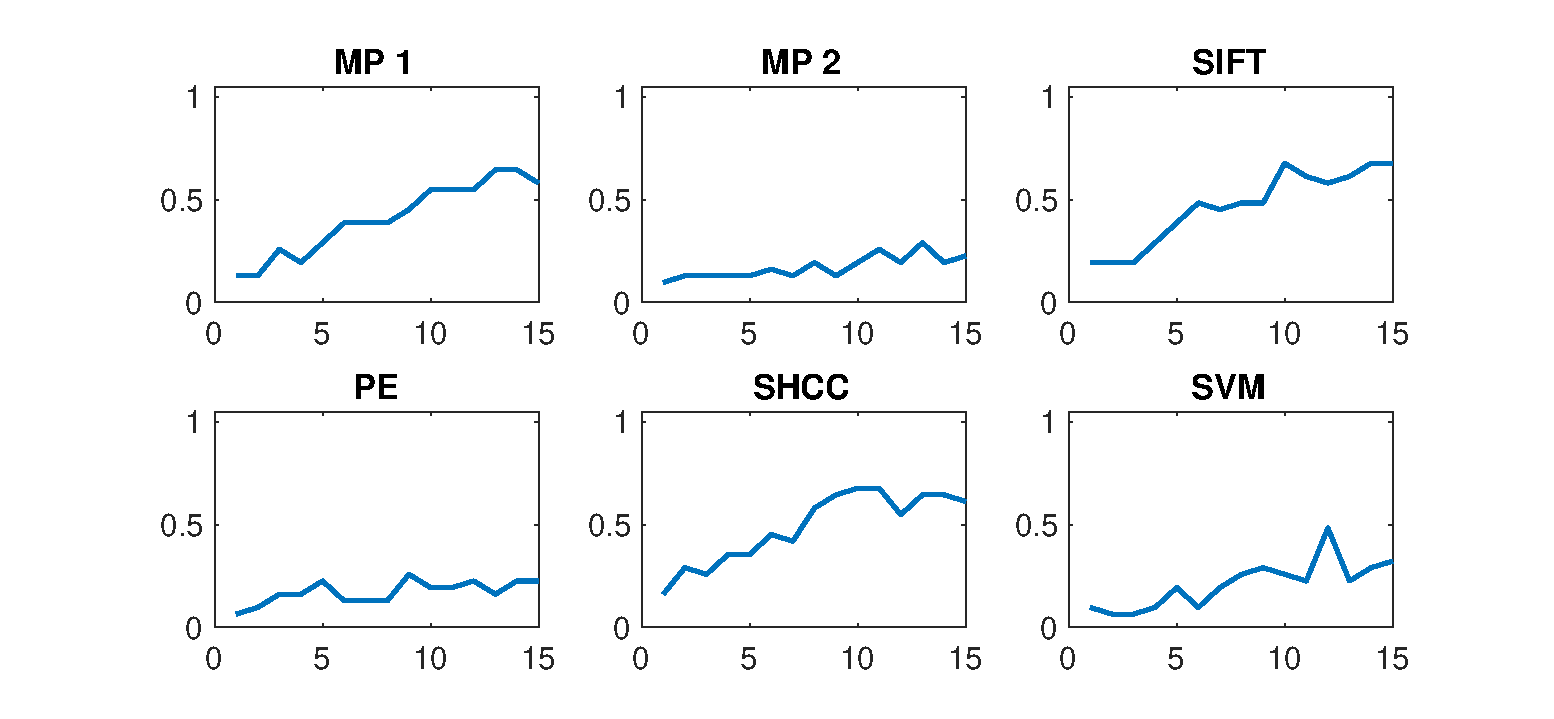
\includegraphics[width=15cm]{images/PerformanceBCICompetition.eps}
\caption[Dataset IIb BCI Competition II (2003) Speller Performance]{Speller performance obtained for the Dataset IIb of the BCI Competition II (2003) for each one of the algorithms.  An offline BCI Simulation is performed using the first $42$ trials as training and the remaining $31$ as testing.  The horizontal axis show the number of intensification sequences, from $0$ to $15$ for this dataset, while the vertical axis show the performance rate.}
\label{fig:performancebcicompetition}
\end{figure}

\section{Conclusion}

%In this paper, a new unsupervised method to enhance evoked response by target stimuli in an oddball paradigm was presented. Only given the time indexes of rows/columns intensifications, the proposed algorithm estimates the main components of the P300 subspace by providing the best SNR. It was shown to efficiently improve the quality of the evoked responses by taking into account the signal and the noise, as opposed to principal component analysis, which only considers the signal. Using this method to enhance P300 subspace before the BCI classification task speeds up the BCI since less words are required to train the spatial filters and the linear classifier, given a certain percentage of good symbol prediction. Moreover, using this spatial enhancement significantly reduces the dimension of the feature vector used to predict words.

%For both datasets, the experimental protocol uses a very short inter-stimulus interval which has the potential to increase the ITR but at the same time it reduces the amplitude of the P300 response, hence it may be more difficult to detect it~\cite{Rao2013}.   It is known that ISI alters the P300 amplitude and may affect the chance to detect the ERP.

%In the case of the P300 response, the oddball paradigm requires that one of the stimuli be infrequent. Hence this forces the data to be unbalanced~\cite{Tibon2015}.  At the same time, the NBNN method suffers from biased classification on unbalanced classes~\cite{Fornoni2014}. %Para solucionar este problema, 

The usage of the Histogram of Gradient Orientations to implement a valid P300-Based BCI Speller application is expounded.  Additionally, its validity is, first, evaluated using a public dataset of ALS patients and an own dataset of healthy subjects.  Second, the method is contrasted against other approaches based on a shared similar idea and results are presented.  Finally, the method is used on a public dataset of a BCI Competition.

%The method works on a channel by channel basis; in this way the best performing channel can be identified and used it to reduce the number of required EEG electrodes, leading to the development of more ergonomic capturing device.

It is verified that this method has an improved performance at letter identification than other methods that process the signals on a channel by channel strategy, and it even has a comparable performance against other methods like SWLDA or SVM, which uses a multichannel feature.
Furthermore, this method has the advantage that shapes of waveforms can be analyzed in an objective way.  We observed that the shape of the P300 component is more stable in occipital channels, where the performance for identifying letters is higher.   We additionally verified that ALS P300 signatures are stable in comparison to those of healthy subjects.

%Further work should be conducted over larger samples to cross-check the validity of these results.

We believe that the use of descriptors based on the histogram of gradient orientation, presented in this work, can also be utilized for deriving a shape metric in the space of the P300 signals which can complement other metrics based on time-domain as those defined by~\cite{Mak2012}. It is important to notice that the analysis of these waveform shapes is usually performed in a qualitative approach based on visual inspection~\cite{SellersandEmanuelDonchin2006}, and a complementary methodology which offer a quantitative metric will be beneficial to these routinely analysis of the waveform of ERPs.

%and, based on this idea, we wanted to complement the methodology with a cuantitative and objective sight

Considering other methods inspired on the same idea, we verified that similar performance results are obtained for the methods \textit{SHCC}, \textit{SIFT} and \textit{MP-1} and that it is also possible to obtain discriminating information from the underlying signal based exclusively on an automated method of processing the waveforms.  Moreover, the possibilities of finding overcomplete dictionaries for matching pursuit sparse representation based on obtained signal templates, could also be considered an area of future improvement~\cite{Gribonval2008}.

The goal of this Chapter is to answer the question if a P300 component could be solely determined by inspecting automatically their waveforms.  We conclude affirmatively, though two very important issues still remain:

First, the stability of the P300 in terms of its shape is crucial: the averaging procedure, montages, the signal to noise ratio and spatial filters all of them are non-physiological factors that affect the stability of the shape of the P300 ERP.  We tested a preliminary approach to assess if the morphological shape of the P300 of the averaged signal can be stabilized by applying different alignments of the stacked segments (see Figure~\ref{fig:classification}) and we verified that there is a better performance when a correct segment alignment is applied.  We applied Dynamic Time Warping (DTW)~\cite{Casarotto2005} to automate the alignment procedure but we were unable to find a substantial improvement.  Further work to study the stability of the shape of the P300 signature component needs to be addressed.

The second problem is the amplitude variation of the P300. We propose a solution by standardizing the signal, shown in Equation~\ref{eq:standarizedaverages}. It has the effect of normalizing the peak-to-peak amplitude, moderating its variation. It has also the advantage of reducing noise that was not reduced by the averaging procedure.   It is important to remark that the averaged signal variance depends on the number of segments used to compute it \cite{van2006signal}.  The standardizing process converts the signal to unit signal variance which makes it independent of the number $k_a$ of signals averaged.   Although this is initially an advantageous approach, the standardizing process reduces the amplitude of any significant P300 complex diminishing its automatic interpretation capability.


%The spelled words are \textit{GATTO}, \textit{MENTE}, \textit{VIOLA} and \textit{REBUS}.

%The purpose of this work is threefold, (1) raise awareness about the utility of using automatic waveform-based methods to study EEG signals, (2) to provide an overview of the state-of-the-art of those methods, and (3) to compare those methods and verify if it is possible to obtain acceptable classification performances based exclusively on the signal's waveform.
